%~~~~~~~~~~~~~~~~~~~~~~~~~~~~~~~~~~~~~~~~~~~~~~~~~~~~~~~~~~~~~~~~~~~~~~~~~~~~~~~~~~~~~~~~~
% Official IISER Thiruvananthapuram Thesis/Dissertation Format
% LaTeX Template for Overleaf
%
% Copyright (c) 2022 by Nikhil Alex
%
% Licensed under Creative Commons Attribution–NonCommercial–ShareAlike 4.0
% (CC BY-NC-SA 4.0). More info: https://creativecommons.org/licenses/by-nc-sa/4.0/
%
% Suggestions/Feedback: nikhil.alexv17@alumni.iisertvm.ac.in
%~~~~~~~~~~~~~~~~~~~~~~~~~~~~~~~~~~~~~~~~~~~~~~~~~~~~~~~~~~~~~~~~~~~~~~~~~~~~~~~~~~~~~~~~~

% Comments like this begin with a % character. 
% Ctrl+b for \textbf{bold} and Ctrl+i for \textit{italics} 
% Ctrl+/ to comment out lines

%=========================================================================================
% PREAMBLE (PACKAGES AND DOCUMENT CONFIGURATION)
%=========================================================================================

% Rewrite the input fields marked with [] brackets.
% Read all uncommented lines carefully.

%~~~~~~~~~~~~~~~~~~~~~~~~~~~~~~~~~~~~~~~~~~~~~~~~~~~~~~~~~~~~~~~~~~~~~~~~~~~~~~~~~~~~~~~~~

\documentclass[12pt,twoside,a4paper]{report} % Font size (pt)
% Add in draft parameter to hide non-essential elements for faster compile times

% Load configuration files
%=========================================================================================
% PACKAGES — ORGANIZED BY CATEGORY
%=========================================================================================

%-----------------------------------------------------------------------------------------
% MATH & SYMBOLS
%-----------------------------------------------------------------------------------------

\usepackage{amsmath}       % Core AMS math features
\usepackage{amsfonts}      % Math fonts
\usepackage{amssymb}       % Extended math symbols
\usepackage{amsthm}        % Theorem and proof environments
\usepackage{mathrsfs}      % Script-style math fonts
\usepackage{yhmath}        % Wide accents
\usepackage{empheq}        % Highlight/emphasise equations
\usepackage{bm}            % Bold math symbols
\usepackage{mathtools}     % Enhancements to amsmath
\usepackage{nccmath}       % Compact math environments 

%-----------------------------------------------------------------------------------------
% DOCUMENT LAYOUT
%-----------------------------------------------------------------------------------------

\usepackage{setspace}      % Line spacing control
\usepackage{geometry}      % Page size and margin settings
\geometry{
    a4paper,               % Paper size
    centering,
    left=1.25in,           % Margins
    right=1in,
    top=0in+1in,
    bottom=1in
}

%-----------------------------------------------------------------------------------------
% REFERENCES & LINKS
%-----------------------------------------------------------------------------------------

\usepackage{hyperref}      % Clickable links and cross-references

\hypersetup{
    colorlinks,
    linkcolor={blue!50!black},
    citecolor={blue!50!black},
    urlcolor={blue!80!black},
    pdfpagelayout=TwoPageRight         
}
\usepackage[backend=biber,style=verbose]{biblatex} % Bibliography
% (See https://tug.ctan.org/info/biblatex-cheatsheet/biblatex-cheatsheet.pdf)
\usepackage[nottoc]{tocbibind}   % Add LoF/LoT to TOC
\usepackage{appendix}      % Appendix formatting
\addbibresource{ref.bib}

%-----------------------------------------------------------------------------------------
% TABLES & FIGURES
%-----------------------------------------------------------------------------------------

\usepackage{caption}       % Custom captions
\usepackage{booktabs}      % Professional tables
\usepackage{graphicx}      % Include graphics
\graphicspath{{./Images/}} % Figures directory
\usepackage{multicol}      % Multiple columns
\usepackage{longtable}     % Multi-page tables

%-----------------------------------------------------------------------------------------
% HEADERS / FOOTERS
%-----------------------------------------------------------------------------------------

\usepackage{fancyhdr}      % Custom headers and footers
% \pagestyle{fancy}        % Enable for standard header and footer

%-----------------------------------------------------------------------------------------
% DATE FORMATTING
%-----------------------------------------------------------------------------------------

\usepackage[UKenglish,cleanlook]{isodate}

%-----------------------------------------------------------------------------------------
% COLORS
%-----------------------------------------------------------------------------------------

\usepackage{xcolor}        % Colors

%-----------------------------------------------------------------------------------------
% DRAWING & GRAPHICS
%-----------------------------------------------------------------------------------------

\usepackage{tikz}          % Drawing diagrams
\newcommand\fillin[1][3cm]{\makebox[#1]{\dotfill}} % Dotted Line

%-----------------------------------------------------------------------------------------
% CHEMICAL NOTATION
%-----------------------------------------------------------------------------------------

% \usepackage[version=4]{mhchem} % Chemical formulae and equations
% \usepackage{chemfig}     % Molecule structural formulae
% \usepackage{chemformula} % Chemical notations with more customisation

%-----------------------------------------------------------------------------------------
% OPTIONAL PACKAGES (UNCOMMENT TO ENABLE)
%-----------------------------------------------------------------------------------------

% \usepackage{xwatermark}  % Watermark
% \usepackage{tikz-cd}     % Commutative diagrams
% \usepackage{pgfplots}    % 2D/3D plots
% \usepackage{footmisc}    % Advanced footnotes
% \usepackage{nomencl}     % List of symbols
% \usepackage{makeidx}     % Index
% \usepackage{enumitem}    % Custom lists
% \usepackage{aliascnt}    % Multiple theorem counters
% \usepackage{mdframed}    % Colored/shaded boxes
% \usepackage{psfrag}      % Replace text in EPS
% \usepackage{fontawesome}       % Icon pack (X, FB, ORCID, etc.)
% \usepackage{siunitx}     % Typeset units
% \usepackage{units}       % Typeset units (Legacy)
% \usepackage[english]{babel}    % Language settings
% \usepackage{verbatim}    % Display long code blocks
% \usepackage[l3]{csvsimple}     % CSV table import

%=========================================================================================
% CUSTOM SETTINGS & ENVIRONMENTS
%=========================================================================================

% Chapter and Section Headings in Headers
\renewcommand{\chaptermark}[1]{\markboth{#1}{}}
\renewcommand{\sectionmark}[1]{\markright{\thesection\ #1}}

% Spacing
\setlength{\parskip}{1em plus 0.25em minus 0.25em}
\renewcommand{\baselinestretch}{1.2}

% Theorem Environments
\theoremstyle{plain}
\newtheorem{theorem}{Theorem}[section]
\newtheorem{lemma}[theorem]{Lemma}
\newtheorem{corollary}[theorem]{Corollary}
\newtheorem{proposition}[theorem]{Proposition}
\theoremstyle{definition}
\newtheorem{definition}[theorem]{Definition}
\newtheorem{example}[theorem]{Example}
\newtheorem{notation}[theorem]{Notation}
\theoremstyle{remark}
\newtheorem{remark}[theorem]{Remark}

% Autoref Naming
\providecommand*{\definitionautorefname}{Definition}
\providecommand*{\propositionautorefname}{Proposition}
\providecommand*{\theoremautorefname}{Theorem}
\providecommand*{\corollaryautorefname}{Corollary}
\providecommand*{\lemmaautorefname}{Lemma}

%-----------------------------------------------------------------------------------------
% OTHER DOCUMENT METADATA
%-----------------------------------------------------------------------------------------

\newcommand{\RegNumber}{[Registration Number]}
\newcommand{\Degree}{}
\newcommand{\Department}{[Department Name]}
\newcommand{\ProjectSupervisor}{[Project Supervisor]}
\newcommand{\ThesisCommitteeMemberA}{[TC Member 1]}
\newcommand{\TCMAFacultyPosition}{[Faculty Position]}
\newcommand{\ThesisCommitteeMemberB}{[TC Member 2]}
\newcommand{\TCMBFacultyPosition}{[Faculty Position]}
\newcommand{\ThesisCommitteeMemberC}{[TC Member 3]}
\newcommand{\TCMCFacultyPosition}{[Faculty Position]}

% Hyperref PDF metadata
\newcommand{\ThesisAuthor}{John Doe}
\newcommand{\ThesisTitle}{My Thesis Title}
\newcommand{\ThesisSubject}{\Degree\ Thesis, IISER Thiruvananthapuram}
\newcommand{\ThesisKeywords}{IISER Thiruvananthapuram}

%----------------- Input Commands -----------------%

\newcommand{\SetThesisTitle}[1]{\renewcommand{\ThesisTitle}{#1}}
\newcommand{\SetThesisAuthor}[1]{\renewcommand{\ThesisAuthor}{#1}}
\newcommand{\SetThesisSubject}[1]{\renewcommand{\ThesisSubject}{#1}}
\newcommand{\SetRegNumber}[1]{\renewcommand{\RegNumber}{#1}}
\def\msc{MSc}
\def\phd{PhD}
\def\minor{Minor}
\newcommand{\SetDegree}[1]{%
    \let\Degree=#1%
    \def\DegreeDisplay{}%
    \edef\tempDegree{#1}%
    \ifx\tempDegree\msc
        \def\DegreeDisplay{Master of Science}%
    \else
        \ifx\tempDegree\phd
            \def\DegreeDisplay{Doctor of Philosophy}%
        \else
            \ifx\tempDegree\minor
                \def\DegreeDisplay{Minor Degree}%
            \else
                \def\DegreeDisplay{#1}%
            \fi
        \fi
    \fi
}
\newcommand{\SetDepartment}[1]{\renewcommand{\Department}{#1}}
\newcommand{\SetProjectSupervisor}[1]{\renewcommand{\ProjectSupervisor}{#1}}
\newcommand{\SetThesisCommitteeMemberA}[1]{\renewcommand{\ThesisCommitteeMemberA}{#1}}
\newcommand{\SetTCMAFacultyPosition}[1]{\renewcommand{\TCMAFacultyPosition}{#1}}
\newcommand{\SetThesisCommitteeMemberB}[1]{\renewcommand{\ThesisCommitteeMemberB}{#1}}
\newcommand{\SetTCMBFacultyPosition}[1]{\renewcommand{\TCMBFacultyPosition}{#1}}
\newcommand{\SetThesisCommitteeMemberC}[1]{\renewcommand{\ThesisCommitteeMemberC}{#1}}
\newcommand{\SetTCMCFacultyPosition}[1]{\renewcommand{\TCMCFacultyPosition}{#1}}
\newcommand{\SetThesisKeywords}[1]{\renewcommand{\ThesisKeywords}{#1}}

%=========================================================================================
% ABBREVIATIONS, CONSTANTS, SYMBOLS LISTS FOR GLOSSARY
%=========================================================================================

% Abbreviations
\newcommand\listsymbolname{Abbreviations}
\newcommand\listofsymbols[2]{
  \section*{\listsymbolname}
  \addcontentsline{toc}{section}{\listsymbolname}
  \begin{longtable}[c]{#1}
    #2
  \end{longtable}\par
}

% Constants
\newcommand\listconstants{Physical Constants}
\newcommand\listofconstants[2]{
  \section*{\listconstants}
  \addcontentsline{toc}{section}{\listconstants}
  \begin{longtable}[c]{#1}
    #2
  \end{longtable}\par
}

% Symbols (Nomenclature)
\newcommand\listnomenclature{Symbols}
\newcommand\listofnomenclature[2]{
  \section*{\listnomenclature}
  \addcontentsline{toc}{section}{\listnomenclature}
  \begin{longtable}[c]{#1}
    #2
  \end{longtable}\par
}      % Packages, layout, spacing, theorem styles
% Set custom colours here:

\definecolor{mygrey}{RGB}{243,243,243}
       % Colour definitions
%=========================================================================================
% MATH SHORTHANDS
%=========================================================================================
\DeclarePairedDelimiter{\abs}{\lvert}{\rvert}
\DeclarePairedDelimiter{\norm}{\lVert}{\rVert}
\DeclarePairedDelimiter\ceil{\lceil}{\rceil}
\DeclarePairedDelimiter\floor{\lfloor}{\rfloor}
\newcommand{\reals}{\mathbb{R}}
\newcommand{\complex}{\mathbb{C}}
\newcommand{\rational}{\mathbb{Q}}
\newcommand{\integers}{\mathbb{Z}}
\newcommand{\naturals}{\mathbb{N}}
\newcommand{\jacobian}{\mathcal{J}}
\newcommand{\bigzero}{\mathbf{0}}
\newcommand{\ds}{\displaystyle}
\newcommand{\Ll}{\mathbb{L}}
\newcommand{\la}{\lambda}
\newcommand{\cof}{\textup{cof }}
\newcommand{\dsum}{\displaystyle\sum}
\newcommand{\1}{\mathbf 1}

%=========================================================================================
% BLACKBOARD BOLD (Sets, Fields, etc.)
%=========================================================================================
\newcommand{\R}{\mathbb{R}}
\newcommand{\N}{\mathbb{N}}
\newcommand{\Z}{\mathbb{Z}}
\newcommand{\F}{\mathbb{F}}
\newcommand{\Q}{\mathbb{Q}}
\newcommand{\C}{\mathbb{C}}
\newcommand{\T}{\mathbb{T}}

\newcommand{\bbA}{\mathbb{A}}
\newcommand{\bbB}{\mathbb{B}}
\newcommand{\bbC}{\mathbb{C}}
\newcommand{\bbD}{\mathbb{D}}
\newcommand{\bbE}{\mathbb{E}}
\newcommand{\bbF}{\mathbb{F}}
\newcommand{\bbG}{\mathbb{G}}
\newcommand{\bbH}{\mathbb{H}}
\newcommand{\bbI}{\mathbb{I}}
\newcommand{\bbJ}{\mathbb{J}}
\newcommand{\bbK}{\mathbb{K}}
\newcommand{\bbL}{\mathbb{L}}
\newcommand{\bbM}{\mathbb{M}}
\newcommand{\bbN}{\mathbb{N}}
\newcommand{\bbO}{\mathbb{O}}
\newcommand{\bbP}{\mathbb{P}}
\newcommand{\bbQ}{\mathbb{Q}}
\newcommand{\bbR}{\mathbb{R}}
\newcommand{\bbS}{\mathbb{S}}
\newcommand{\bbT}{\mathbb{T}}
\newcommand{\bbU}{\mathbb{U}}
\newcommand{\bbV}{\mathbb{V}}
\newcommand{\bbW}{\mathbb{W}}
\newcommand{\bbX}{\mathbb{X}}
\newcommand{\bbY}{\mathbb{Y}}
\newcommand{\bbZ}{\mathbb{Z}}

%=========================================================================================
% CALLIGRAPHIC LETTERS
%=========================================================================================
\newcommand{\cA}{\mathcal{A}}
\newcommand{\cB}{\mathcal{B}}
\newcommand{\cC}{\mathcal{C}}
\newcommand{\cD}{\mathcal{D}}
\newcommand{\cE}{\mathcal{E}}
\newcommand{\cF}{\mathcal{F}}
\newcommand{\cG}{\mathcal{G}}
\newcommand{\cH}{\mathcal{H}}
\newcommand{\cI}{\mathcal{I}}
\newcommand{\cJ}{\mathcal{J}}
\newcommand{\cK}{\mathcal{K}}
\newcommand{\cL}{\mathcal{L}}
\newcommand{\cM}{\mathcal{M}}
\newcommand{\cN}{\mathcal{N}}
\newcommand{\cO}{\mathcal{O}}
\newcommand{\cP}{\mathcal{P}}
\newcommand{\cQ}{\mathcal{Q}}
\newcommand{\cR}{\mathcal{R}}
\newcommand{\cS}{\mathcal{S}}
\newcommand{\cT}{\mathcal{T}}
\newcommand{\cU}{\mathcal{U}}
\newcommand{\cV}{\mathcal{V}}
\newcommand{\cW}{\mathcal{W}}
\newcommand{\cX}{\mathcal{X}}
\newcommand{\cY}{\mathcal{Y}}
\newcommand{\cZ}{\mathcal{Z}}

%=========================================================================================
% FRAKTUR LETTERS
%=========================================================================================
\newcommand{\fA}{\mathfrak{A}}
\newcommand{\fB}{\mathfrak{B}}
\newcommand{\fC}{\mathfrak{C}}
\newcommand{\fD}{\mathfrak{D}}
\newcommand{\fE}{\mathfrak{E}}
\newcommand{\fF}{\mathfrak{F}}
\newcommand{\fG}{\mathfrak{G}}
\newcommand{\fH}{\mathfrak{H}}
\newcommand{\fI}{\mathfrak{I}}
\newcommand{\fJ}{\mathfrak{J}}
\newcommand{\fK}{\mathfrak{K}}
\newcommand{\fL}{\mathfrak{L}}
\newcommand{\fM}{\mathfrak{M}}
\newcommand{\fN}{\mathfrak{N}}
\newcommand{\fO}{\mathfrak{O}}
\newcommand{\fP}{\mathfrak{P}}
\newcommand{\fQ}{\mathfrak{Q}}
\newcommand{\fR}{\mathfrak{R}}
\newcommand{\fS}{\mathfrak{S}}
\newcommand{\fT}{\mathfrak{T}}
\newcommand{\fU}{\mathfrak{U}}
\newcommand{\fV}{\mathfrak{V}}
\newcommand{\fW}{\mathfrak{W}}
\newcommand{\fX}{\mathfrak{X}}
\newcommand{\fY}{\mathfrak{Y}}
\newcommand{\fZ}{\mathfrak{Z}}

%=========================================================================================
% AUTOMATIC WIDE HAT DEFINITIONS (UPPERCASE + LOWERCASE)
%=========================================================================================
\usepackage{pgffor} % Required for \foreach loops

% Uppercase letters
\foreach \X in {A,...,Z} {%
    \expandafter\newcommand\csname hat\X\endcsname{\widehat{\X}}%
}

% Lowercase letters
\foreach \x in {a,...,z} {%
    \expandafter\newcommand\csname hat\x\endcsname{\widehat{\x}}%
}   % Math symbols and alphabet macros
%=========================================================================================
% ADDITIONS FOR THIS REPORT
% Everything here is on top of the official template; nothing in Preamble.tex is
% changed. Loaded from Main_Report.tex after the template's own configuration.
%=========================================================================================

%-----------------------------------------------------------------------------------------
% Degree: BS-MS minor project
% The template offers \msc, \phd and \minor, but \minor prints "Minor Degree" (IISER's
% minor-degree programme), which is not what this is. \bsms falls through to the
% template's own "else" branch, so it displays exactly the text below. The title page's
% "A ... Submitted" line has a matching branch in Intro_Pages/01_TitlePage.tex.
%-----------------------------------------------------------------------------------------
\newcommand{\bsms}{BS-MS (Dual Degree)}

%-----------------------------------------------------------------------------------------
% Submission date
% The template prints \today (the day the PDF is compiled). The report states a fixed
% submission month instead, so the front pages do not change every time it is rebuilt.
%-----------------------------------------------------------------------------------------
\newcommand{\SubmissionDate}{November 2026}

%-----------------------------------------------------------------------------------------
% Packages the chapters use that the template does not load
%-----------------------------------------------------------------------------------------
\usepackage{float}                         % [H] placement for tables and figures
\usepackage[nameinlink,capitalise]{cleveref} % \cref / \Cref (must come after hyperref)
\usepackage{listings}                      % the commands in the appendix
\lstset{basicstyle=\ttfamily\small, breaklines=true, frame=single,
        columns=fullflexible, keepspaces=true}
\graphicspath{{./Images/}{./Images/Figures/}}

%-----------------------------------------------------------------------------------------
% House style: spell these the same way everywhere
%-----------------------------------------------------------------------------------------
\newcommand{\tfunet}{\texttt{tf\_unet}}
\newcommand{\hybrid}{HybridRFINet}
\newcommand{\aoflagger}{\textsc{AOFlagger}}
\newcommand{\Fone}{$F_1$}

%-----------------------------------------------------------------------------------------
% Line breaking in the template's narrower text column
%-----------------------------------------------------------------------------------------
\hyphenation{Hybrid-RFI-Net PSR-CHIVE AO-Flagger}
\setlength{\emergencystretch}{1.5em}      % lets awkward lines break without overflowing
\appto{\bibsetup}{\emergencystretch=1em}   % same for long bibliography entries
  % Additions for this report (see file)

% Document Metadata
\SetThesisTitle{Detecting Radio Frequency Interference in Radio Spectrograms with Convolutional Networks}
\SetThesisAuthor{Ronak Singh}
\SetRegNumber{IMS23319}
\SetDegree{\bsms}                        % Choose from: \msc, \phd, and \minor
                                         % (\bsms is defined in ReportExtras.tex: the
                                         %  template's \minor prints "Minor Degree",
                                         %  which is a different programme)
\SetDepartment{Physics}
\SetProjectSupervisor{Alwin Poulose}
\SetThesisCommitteeMemberA{[TC Member 1]}
\SetTCMAFacultyPosition{[Faculty Position]}
\SetThesisCommitteeMemberB{[TC Member 2]}
\SetTCMBFacultyPosition{[Faculty Position]}
\SetThesisCommitteeMemberC{[TC Member 3]}
\SetTCMCFacultyPosition{[Faculty Position]}
\SetThesisKeywords{Radio frequency interference, RFI flagging, U-Net, image segmentation, deep learning, LOFAR}

\hypersetup{
    pdfauthor={\ThesisAuthor},
    pdftitle={\ThesisTitle},
    pdfsubject={\ThesisSubject},
    pdfkeywords={IISER Thiruvananthapuram, \ThesisKeywords}
}

%=========================================================================================
% DOCUMENT STARTS HERE
%=========================================================================================

\begin{document}

%=========================================================================================
% INTRODUCTORY PAGES
%=========================================================================================

\newgeometry{
  inner=45pt,
  outer=48pt,
  top=1.5in
}

%~~~~~~~~~~~~~~~~~~~~~~~~~~~~~~~~~~~~~~~~~~~~~~~~~~~~~~~~~~~~~~~~~~~~~~~~~~~~~~~~~~~~~~~~~%
%	                                     TITLE PAGE	                                      %
%~~~~~~~~~~~~~~~~~~~~~~~~~~~~~~~~~~~~~~~~~~~~~~~~~~~~~~~~~~~~~~~~~~~~~~~~~~~~~~~~~~~~~~~~~%
\begin{titlepage}
\enlargethispage{3cm}

\begin{center}

\vspace*{-1cm}

{\bf \Large \MakeUppercase{\ThesisTitle}}\\[10pt]

\vspace*{0.5cm}

\ifx\Degree\phd
A Thesis Submitted\\
\else
\ifx\Degree\bsms
A Minor Project Report Submitted\\
\else
    \ifx\Degree\minor
    A Minor Project Dissertation Submitted\\
    \else
        A Dissertation Submitted\\
    \fi
\fi
\fi

in Partial Fulfilment of the Requirements  \\
    for the Degree of  \\
    \vspace{0.5cm}

{\Large \bf \MakeUppercase{\DegreeDisplay}}

\vspace{0.3cm}
    in 
\vspace{0.3cm}
{\large \bf \Department } \\

\vspace{10mm}
{\em  by} \\ \vspace{3mm}
{\large \bf \ThesisAuthor} \\
{\large \bf (Reg. No. \RegNumber)}\\[.3in]

\vspace{3cm}

\begin{figure}[h]
  \begin{center}
  
\includegraphics[height=36mm]{Logos/iiser_logo.png}
  \end{center}
\end{figure}
\vspace*{0.2cm}

{\em\large to }\\[8pt]
{\bf\large SCHOOL OF \MakeUppercase{\Department}} \\[4pt]
{\bf \large INDIAN INSTITUTE OF SCIENCE EDUCATION AND RESEARCH}\\%[4pt]
{\bf\large THIRUVANANTHAPURAM}\\[4pt]
{\bf\large INDIA - 695 551}\\[12pt]
{\it\large \SubmissionDate}

\end{center}

\end{titlepage}
\thispagestyle{empty} % Avoid page numbering
\cleardoublepage % Alternate clear pages for a two-sided report

\pagenumbering{roman}
\setcounter{page}{3}
%~~~~~~~~~~~~~~~~~~~~~~~~~~~~~~~~~~~~~~~~~~~~~~~~~~~~~~~~~~~~~~~~~~~~~~~~~~~~~~~~~~~~~~~~~%
%	                                    CERTIFICATE                                  %
%~~~~~~~~~~~~~~~~~~~~~~~~~~~~~~~~~~~~~~~~~~~~~~~~~~~~~~~~~~~~~~~~~~~~~~~~~~~~~~~~~~~~~~~~~%
\begin{center}
{\Large{\bf{CERTIFICATE}}}
\end{center}
% To be signed by thesis committee (TC) members


\noindent
This is to certify that this dissertation entitled {\bf ``\ThesisTitle''}  submitted by {\bf\ThesisAuthor\ (Reg.\ No.:\ \RegNumber)} towards the partial requirement of {\bf \DegreeDisplay} in {\bf \Department}, has been duly examined by the thesis committee appointed by the institute. The committee deems the candidate's work satisfactory and recommends that the report be accepted.

\vspace{3.5cm}

\noindent
\begin{minipage}[l]{0.3\textwidth}
\centering
\fillin[0.9\linewidth]\\
{\large \bf \ThesisCommitteeMemberA} \medskip\\
{\large \TCMAFacultyPosition}
\end{minipage}
\hfill
\begin{minipage}[c]{0.3\textwidth}
\centering
\fillin[0.9\linewidth]\\
{\large \bf \ThesisCommitteeMemberB} \medskip\\
{\large \TCMBFacultyPosition}
\end{minipage}
\hfill
\begin{minipage}[r]{0.3\textwidth}
\centering
\fillin[0.9\linewidth]\\
{\large \bf \ThesisCommitteeMemberC} \medskip\\
{\large \TCMCFacultyPosition}
\end{minipage}

\vspace{4cm}

\begin{flushright}
    \begin{minipage}[c]{0.4\textwidth}
    \centering
    \fillin[0.9\linewidth]\\
    {\large \bf \ProjectSupervisor} \medskip\\
    {\large Project Supervisor}
    \end{minipage}
\end{flushright}
\vfill
\noindent\SubmissionDate \\
Thiruvananthapuram - 695 551
\vspace{1.5cm}
\cleardoublepage

%~~~~~~~~~~~~~~~~~~~~~~~~~~~~~~~~~~~~~~~~~~~~~~~~~~~~~~~~~~~~~~~~~~~~~~~~~~~~~~~~~~~~~~~~~%
%                                       DECLARATION	                                      %
%~~~~~~~~~~~~~~~~~~~~~~~~~~~~~~~~~~~~~~~~~~~~~~~~~~~~~~~~~~~~~~~~~~~~~~~~~~~~~~~~~~~~~~~~~%
\begin{center}
{\Large{\bf{DECLARATION}}}
\end{center}

\noindent
I, {\bf\ThesisAuthor\ (Reg.\ No.:\ \RegNumber)}, hereby declare that this dissertation entitled {\bf``\ThesisTitle”}, submitted to Indian Institute of Science Education and Research, Thiruvananthapuram, towards the partial requirement of {\bf\DegreeDisplay} in {\bf \Department}, is a bona fide record of original work carried out by me under the supervision of {\bf \ProjectSupervisor}. 
\par This dissertation has never been submitted in part or in full for a degree, diploma or fellowship to this or any other university before. I duly acknowledge all external contributions, statements, datasets or results used, and have listed their sources with adequate detail in the bibliography.

\vspace{2.5cm}

\begin{flushright}
    \begin{minipage}[c]{0.4\textwidth}
    \centering
    \fillin[0.9\linewidth]\\
    {\large \bf \ThesisAuthor} \medskip\\
    {\large Reg. No.: \RegNumber}
    \end{minipage}
\end{flushright}
\vspace{0.8cm}
\noindent
In my capacity as the project supervisor for the aforementioned candidate, I confirm that the above statements by the candidate are true to the best of my knowledge.

\vspace{2.5cm}

\begin{flushright}
    \begin{minipage}[c]{0.4\textwidth}
    \centering
    \fillin[0.9\linewidth]\\
    {\large \bf \ProjectSupervisor} \medskip\\
    {\large Project Supervisor}
    \end{minipage}
\end{flushright}
\vfill
\noindent\SubmissionDate \\
Thiruvananthapuram - 695 551
\vspace{1.5cm}
\cleardoublepage

%~~~~~~~~~~~~~~~~~~~~~~~~~~~~~~~~~~~~~~~~~~~~~~~~~~~~~~~~~~~~~~~~~~~~~~~~~~~~~~~~~~~~~~~~~%
%	                                    ACKNOWLEDGEMENT                                   %
%~~~~~~~~~~~~~~~~~~~~~~~~~~~~~~~~~~~~~~~~~~~~~~~~~~~~~~~~~~~~~~~~~~~~~~~~~~~~~~~~~~~~~~~~~%
\begin{center}
{\Large{\bf{ACKNOWLEDGEMENT}}}
\end{center}
%\thispagestyle{empty}


\noindent
[Insert Acknowledgements here \ldots]
% TODO (Ronak): thank your supervisor, the lab and anyone else, in your own words.
\par
Parts of the data analysis, figure generation and drafting support for this
report were carried out with the assistance of Claude (Anthropic). All
experiments, results and conclusions are the author's own.
\par
I am lastly grateful to the Indian Institute of Science Education and Research Thiruvananthapuram for providing the necessary resources and facilities to complete this project to the best of my ability.

\cleardoublepage
%~~~~~~~~~~~~~~~~~~~~~~~~~~~~~~~~~~~~~~~~~~~~~~~~~~~~~~~~~~~~~~~~~~~~~~~~~~~~~~~~~~~~~~~~~%
%	                                     ABSTRACT   	                                  %
%~~~~~~~~~~~~~~~~~~~~~~~~~~~~~~~~~~~~~~~~~~~~~~~~~~~~~~~~~~~~~~~~~~~~~~~~~~~~~~~~~~~~~~~~~%
\begin{flushleft} % This section is not essential for the abstract
    \setlength{\parskip}{0pt}
        %\bigskip
    {\centering{{\Large{\bf{ABSTRACT}}}} \par}
    \medskip
    \vspace{6pt}
    \hrule \vspace{0.4cm}
		  Student Name:	 \textbf{\ThesisAuthor}	\hfill Reg. No.: \textbf{\RegNumber} \\
		Degree:  \textbf{\DegreeDisplay} \hfill Dept.:  \textbf{School of \Department} \\
		Thesis Title: \textbf{\ThesisTitle}\\
		Thesis Supervisor:  \textbf{\ProjectSupervisor}\\
		Date of thesis submission: \textbf{{ \SubmissionDate}\\[0.4cm] }
	\hrule \vspace{1.5cm} 
\end{flushleft}
\noindent
Radio frequency interference (RFI) from human technology corrupts radio
astronomy data and must be flagged before analysis. Treating RFI flagging as
image segmentation, this project reproduces the U-Net method of Akeret et al.\
(\tfunet{}), designs an improved network, and tests both on a synthetic
dataset and on real LOFAR observations labelled by a human expert. On synthetic
data \tfunet{} first scored an \Fone{} of 0.39; controlled experiments traced this
to class weighting combined with its ReLU output layer and to per-image
normalisation, and correcting both raised it to 0.93 without changing the
network. On real LOFAR data, the improved network, \hybrid{}, reaches a maximum
\Fone{} of $0.6603 \pm 0.0040$ with 593{,}842 parameters, above the best published
result of 0.5979. However, removing the components it was designed around---strip
convolutions, channel attention and residual blocks---leaves its score
unchanged, and a conditional random field refinement adds nothing. Checking the
public datasets revealed test images duplicated in the training sets of both
HERA and LOFAR, and the same network scores 0.44 lower on real data than on
synthetic data. The results show that synthetic benchmarks and single training
runs can both mislead, and that claims about why a model works need to be
tested directly.

\vspace{4cm}

{\large \textbf{Keywords: }}\par{\Large \ThesisKeywords}

\cleardoublepage
%~~~~~~~~~~~~~~~~~~~~~~~~~~~~~~~~~~~~~~~~~~~~~~~~~~~~~~~~~~~~~~~~~~~~~~~~~~~~~~~~~~~~~~~~~%
%                   TABLE OF CONTENTS, LIST OF FIGURES, LIST OF TABLES                    %
%~~~~~~~~~~~~~~~~~~~~~~~~~~~~~~~~~~~~~~~~~~~~~~~~~~~~~~~~~~~~~~~~~~~~~~~~~~~~~~~~~~~~~~~~~%

\tableofcontents
\clearpage
\listoffigures
\listoftables

\newpage
%%~~~~~~~~~~~~~~~~~~~~~~~~~~~~~~~~~~~~~~~~~~~~~~~~~~~~~~~~~~~~~~~~~~~~~~~~~~~~~~~~~~~~~~~~~%
%                                            GLOSSARY                                     %
%~~~~~~~~~~~~~~~~~~~~~~~~~~~~~~~~~~~~~~~~~~~~~~~~~~~~~~~~~~~~~~~~~~~~~~~~~~~~~~~~~~~~~~~~~%

\clearpage
{\Huge \bfseries Glossary}
\\[6pt]

\listofsymbols{ll}{
\textbf{FEA} & \textbf{F}inite \textbf{E}lement \textbf{A}nalysis \\
\textbf{FEM} & \textbf{F}inite \textbf{E}lement \textbf{M}ethod \\
\textbf{RC}  & \textbf{R}einforced \textbf{C}oncrete \\
}

\listofconstants{lrcl}{
Speed of Light & $c$ & = & $2.99792458 \times 10^{8}\ \mathrm{m/s}$ (exact) \\
Planck Constant & $h$ & = & $6.62607015 \times 10^{-34}\ \mathrm{J\,s}$ (exact) \\
}

\listofnomenclature{lll}{
$D^{el}$ & Elasticity tensor & Pa \\
$\sigma$ & Stress tensor     & Pa \\
$\varepsilon$ & Strain tensor & - \\
}         % Uncomment to enable glossary page   
\restoregeometry
% Set main page numbering
\pagenumbering{arabic}
\setcounter{page}{1}

%=========================================================================================
% MAIN CHAPTERS
%=========================================================================================

\chapter{Introduction}
\label{ch:intro}

\section{Radio frequency interference}
Radio telescopes detect extremely faint signals from space. The same frequency
bands are also used by human technology: mobile phone towers, satellites,
aircraft and weather radar, television and radio broadcasts, and electrical
equipment such as power lines and car spark plugs. Signals from these sources
leak into the telescope and are usually many orders of magnitude stronger than
the astronomical signal. This is radio frequency interference (RFI).

RFI is different in character from the ordinary noise in a radio observation.
The thermal noise of the receiver and the sky is random and close to Gaussian,
and its statistics are well understood. RFI is not: it is strong, it has
structure in time and frequency, and it changes during an observation. It is
non-Gaussian and non-stationary. Before any scientific analysis, the parts of
the data affected by RFI have to be found and removed, a step called RFI
flagging. Modern telescopes produce far too much data for this to be done by
hand, so it must be automatic.

\section{Motivation: pulsar timing}
This project started from pulsar observations with the upgraded Giant
Metrewave Radio Telescope (uGMRT) in India. Pulsars are rotating neutron stars
that emit very regular pulses; millisecond pulsars are regular enough to be
used as precise clocks. The Indian Pulsar Timing Array (InPTA) times such
pulsars to search for low-frequency gravitational waves, which requires the
arrival times of the pulses to be measured to better than a microsecond. RFI
that is not removed distorts the measured pulse profiles and therefore the
arrival times. The 300--500\,MHz band used by uGMRT is heavily affected by
terrestrial RFI.

The tools commonly used to clean folded pulsar data, such as \texttt{paz}
from PSRCHIVE\footcite{vanstraten2012psrchive} and \texttt{clfd}\footcite{clfd}, rely
on simple statistics such as median filters. Because RFI is non-Gaussian, these
can miss weak broadband RFI or, if made more aggressive, remove parts of the
real pulsar signal.

\section{RFI flagging as image segmentation}
Radio data can be arranged as a two-dimensional image with frequency along one
axis and time along the other, a spectrogram. For folded pulsar data, a
similar image is formed from a statistic of the pulse profile (such as its root
mean square) in each frequency channel and time sub-integration. In this
picture RFI appears as lines, bands and patches, and flagging means deciding,
for every pixel, whether it is affected by RFI. This is the problem that
computer vision calls semantic segmentation.

The U-Net\footcite{ronneberger2015} is a standard neural network for segmentation,
and Akeret et al.\footcite{akeret2017} were the first to apply it to RFI, in a
code called \tfunet{}. A different approach is the 2$\sigma$CRF method of Chen
et al.\footcite{chen2023}, which labels pixels with a statistical threshold and
then refines the labels with a conditional random field (CRF) that takes each
pixel's neighbours into account.

\section{Aims}
The original plan was to combine the two ideas: a U-Net for segmentation,
followed by a CRF to refine its output. The work was carried out on a
synthetic dataset I generated, and then on public datasets from HERA and
LOFAR. The aims were:
\begin{enumerate}
  \item to reproduce the U-Net method of Akeret et al.\ on our own data;
  \item to understand why it initially performed poorly, and correct it;
  \item to design an improved network for RFI;
  \item to test both on real telescope data with labels checked by a human
    expert, not only on synthetic data;
  \item to find out what actually makes the improved network better, including
    whether the CRF step helps.
\end{enumerate}

\section{Summary of results}
\begin{itemize}
  \item \tfunet{} initially scored an \Fone{} of 0.39 on synthetic data. The
    cause was two training settings---class weighting combined with the
    network's output layer, and per-image normalisation---not its
    architecture. Correcting them raised the score to 0.93 without changing the
    network (\cref{ch:tfunet}).
  \item On real LOFAR data with human labels, my network, \hybrid{}, reaches
    a maximum \Fone{} of $0.6603 \pm 0.0040$ with 593{,}842 parameters, above the
    best published result on this data, 0.5979\footcite{mesarcik2022}
    (\cref{ch:hybrid}).
  \item The components the network was designed around contribute nothing
    measurable to this result, and a CRF refinement does not improve it
    (\cref{ch:drivers}).
  \item Checking the public datasets revealed that test images also appear in
    the training set: 31 of 140 in HERA and all 109 in LOFAR
    (\cref{ch:datasets}).
  \item The same network that scores 0.93 on synthetic data scores 0.49 on real
    data under identical settings, showing how much synthetic benchmarks can
    overstate real performance (\cref{sec:gap}).
\end{itemize}

\section{Structure of this report}
\Cref{ch:background} introduces RFI in spectrograms, existing flagging methods
and the evaluation measures used. \Cref{ch:datasets} describes the four
datasets. \Cref{ch:tfunet} reproduces and diagnoses \tfunet{}, and
\cref{ch:hybrid} presents \hybrid{}. \Cref{ch:drivers} tests what drives its
performance, \cref{ch:discussion} discusses the results and their limitations,
and \cref{ch:conclusion} concludes.

\chapter{Background}
\label{ch:background}

\section{RFI in spectrograms}
\label{sec:rfi_types}
In a spectrogram, different kinds of RFI leave different shapes, depending on
how long they last and how many frequencies they cover.
\begin{itemize}
  \item \textbf{Constant narrowband RFI} affects a single frequency channel for
    the whole observation and appears as a thin line along the time axis.
    Typical sources are fixed terrestrial transmitters, such as a particular
    radio or television station.
  \item \textbf{Constant broadband RFI} covers a wide range of frequencies for the
    whole observation and appears as a thick band. Continuously broadcasting
    satellites are a common cause.
  \item \textbf{Instantaneous wideband RFI} lasts only a moment but covers almost
    all frequencies, appearing as a thin line along the frequency axis.
    Lightning, arcing on power lines and radar sweeps produce this kind.
  \item \textbf{Patchy broadband RFI} covers several channels for a few minutes
    and then fades, appearing as irregular, cloud-like patches.
\end{itemize}
Not every structure in a spectrogram is RFI. The receiver's sensitivity
varies with frequency (the bandpass, \cref{sec:bandpass}), and slow drifts and
standing waves add smooth patterns. A flagging method has to distinguish these
from real interference.

\section{Classical flagging methods}

\subsection{Statistical thresholds}
The simplest approach flags any pixel more than $k$ standard deviations above
the mean. Tools used for folded pulsar data, such as \texttt{paz} and
\texttt{clfd}, are based on robust statistics of this kind, such as medians.
They need no training, but they assume the clean data is close to Gaussian, so
they miss faint RFI and struggle when the noise level changes across the data.
On the LOFAR test data, the best simple threshold of this kind reaches an
\Fone{} of 0.41 (\cref{sec:tfunet_lofar}).

\subsection{AOFlagger}
\aoflagger{}\footcite{offringa2012} is the standard RFI flagger for LOFAR. It
combines thresholding at several scales with a morphological step that
extends flags along time and frequency, so that the edges of RFI features are
also caught. It is important for this report because it produced the
training labels of the LOFAR dataset (\cref{sec:lofar}).

\subsection{The 2\texorpdfstring{$\sigma$}{-sigma}CRF method}
Chen et al.\footcite{chen2023} clean RFI in folded pulsar data in two steps.
First, they compute the root-mean-square of the folded profile in each
frequency channel and time sub-integration, giving a 2D image, remove its
baseline, and fit a Gaussian to the histogram of its values. Pixels within
$2\sigma$ of the Gaussian peak are labelled clean, pixels beyond $3\sigma$ are
labelled RFI, and those in between are left ambiguous. Second, they refine
these labels with a fully connected conditional random field
(CRF)\footcite{krahenbuhl2011}. A CRF treats every pixel as connected to the
others and finds the labelling that minimises an energy made of two parts: a
unary term, how likely each pixel is to be RFI on its own, and a pairwise
term, which encourages pixels that are close together and similar in value to
share a label. This lets weak RFI that is unrecognisable in a single pixel be
picked out from its neighbourhood. They report 93--95\% accuracy on data from
the FAST telescope. The method still rests on a Gaussian model of the clean
data, which is where a learned approach might do better.

\section{Neural networks for RFI segmentation}

\subsection{U-Net}
The U-Net\footcite{ronneberger2015} is a convolutional network for image
segmentation. Its encoder repeatedly applies convolutions and halves the image
size, building up a description of \emph{what} is in the image; its decoder
reverses this, restoring the full size to locate \emph{where} it is. Skip
connections pass fine detail directly from each encoder level to the matching
decoder level. The output has one probability per pixel---here, the
probability that the pixel is affected by RFI.

\subsection{\tfunet{}}
Akeret et al.\footcite{akeret2017} applied a U-Net to RFI in their \tfunet{}
code, written in TensorFlow. The configuration used in this report has 3
levels and 32 filters in the first layer, giving 465{,}986 trainable
parameters. Two design details become important later: \tfunet{} applies a ReLU
to its output scores, and it has no normalisation layers
(\cref{ch:tfunet}).

\subsection{Recent methods}
Mesarcik et al.\footcite{mesarcik2022}, who released the LOFAR dataset used here,
proposed an approach called Nearest-Latent-Neighbours, which learns only from
RFI-free data and flags whatever looks unusual. They compared it with several
supervised networks on the same LOFAR test set. The best \Fone{} in their
comparison came from RFI-Net\footcite{yang2020rfinet}, a residual U-Net, with
0.5979; their own U-Net reached $0.5876 \pm 0.0031$. Their method had the best
area under the ROC curve but a lower \Fone{} of 0.5114. These published values
are the benchmarks used in \cref{ch:hybrid}.

\section{Measuring performance}
\label{sec:metrics}
For each pixel, a flagging method either flags it as RFI or not, and it either
is or is not RFI in the reference labels. Counting the true positives (TP),
false positives (FP) and false negatives (FN) over all test pixels gives
\begin{equation}
  \text{precision} = \frac{TP}{TP + FP}, \qquad
  \text{recall} = \frac{TP}{TP + FN}, \qquad
  F_1 = \frac{2\,\text{precision}\cdot\text{recall}}{\text{precision} + \text{recall}}.
\end{equation}
Precision is the fraction of flagged pixels that really are RFI; recall is the
fraction of RFI that was found. \Fone{} is high only if both are.

Accuracy, the fraction of pixels classified correctly, is not useful here.
RFI covers less than 1\% of the LOFAR test pixels, so a method that flags
nothing at all is 99.23\% accurate while finding no RFI.

The area under the ROC curve measures something different: how well a model
\emph{ranks} RFI pixels above clean ones, regardless of where the final cut is
made. A model can rank well and still make poor final decisions
(\cref{sec:hybrid_lofar}).

\paragraph{Choosing the threshold.} A network outputs a probability for each
pixel, and a threshold turns it into a yes/no decision. The choice of threshold
changes the \Fone{}, and there are two ways to make it.
\begin{itemize}
  \item \textbf{Maximum \Fone{}:} try every threshold on the test set and report
    the best. This is optimistic, because it uses the test labels to pick the
    threshold. It is, however, what Mesarcik et al.\ report, so it is needed
    for a fair comparison with their results.
  \item \textbf{Pooled \Fone{}:} choose the threshold on a separate validation
    set, fix it, and then apply it to the test set. This is the honest
    measure of how a model would perform on new data.
\end{itemize}
For example, if a model scores ten pixels and the best threshold on those ten
gives $F_1 = 0.89$, but the threshold chosen beforehand on validation data
gives $0.86$ on the same pixels, the maximum \Fone{} is 0.89 and the pooled
\Fone{} 0.86. The maximum is never lower than the pooled value. In this report
both are given; the pooled value is the one I rely on.

``Pooled'' also means that TP, FP and FN are added up over all test images
before computing a single \Fone{}. Averaging a separate \Fone{} for each image
gives a different number: for \aoflagger{} on LOFAR, the per-image average is
0.103 lower than the pooled value.

\chapter{Datasets}
\label{ch:datasets}
% Opening paragraph: four datasets, two synthetic (ours), two from the
% literature. Only LOFAR has real telescope data with human labels -- say up
% front that this is the one that matters most.

\section{Synthetic dataset}
\label{sec:synthetic}
% Write about your generator. Sources: PART 8, PART 9, "Verified facts"
% section of the context doc, Synthetic Dataset*/dataset_statistics.txt.

\subsection{Generation}
Real radio data with reliable pixel-level RFI labels is scarce, so the first
part of this work used a synthetic dataset that I generated myself. The
generator is written in Python and uses NumPy's random number generator with a
fixed seed (42), so the whole dataset can be regenerated bit for bit.

Each image is a spectrogram: one axis is frequency and the other is time, and
each pixel holds the power received in that frequency channel at that moment.
The background is not plain random noise. It is built from a sky pedestal that
varies across frequency, a smooth astronomical signal, a slow drift in time,
and Gaussian noise on top. RFI is then injected into this background. Six
types of RFI are modelled, chosen to cover the shapes commonly seen in real
observations (\cref{tab:rfi_types}). Each image receives a random selection of
types at random strengths, and images are spread over four density levels:
clean (8.2\%), light (30.0\%), moderate (36.2\%) and heavy (25.6\%).

\begin{table}[H]
  \centering
  \caption{The six RFI types in the synthetic dataset, with the number of the
    1000 images (1024$\times$265 version) that contain each type.}
  \label{tab:rfi_types}
  \begin{tabular}{llr}
    \toprule
    Type & Appearance in the spectrogram & Images \\
    \midrule
    Narrowband      & thin line at one frequency, lasting for some time  & 889 \\
    Scattered       & small isolated hits scattered over the image        & 899 \\
    Blob            & patchy, cloud-like region                           & 673 \\
    Persistent band & group of channels affected for the whole observation & 588 \\
    Broadband block & rectangle covering many channels for a while        & 488 \\
    Wideband burst  & short flash across many channels at once            & 310 \\
    \bottomrule
  \end{tabular}
\end{table}

The dataset contains 1000 images, split into 700 for training, 150 for
validation and 150 for testing. I checked that no image appears in more than
one split by comparing SHA-256 hashes of the raw pixels; there are no shared
hashes.

\subsection{Deciding which pixels are RFI}
\label{sec:synthetic_label}
Because the RFI is injected by the generator, its exact strength at every
pixel is known. A pixel is labelled as RFI when the injected RFI power there
is greater than 0.5 times the standard deviation of the local noise. Pixels
where RFI was added but is weaker than this are labelled clean, because at
that level there is effectively nothing left in the data for a detector to
find.

This rule gives labels that are noise-free and unambiguous: every labelled
pixel is, by construction, measurably above the noise. In the 276$\times$600
version, 90.9\% of the RFI pixels lie at or above one noise standard
deviation. This makes the task considerably easier than labelling real data,
a point that becomes important in \cref{ch:drivers}.

The rule was refined between the two versions of the dataset. In the
276$\times$600 version a pixel was labelled RFI if it lay inside the geometric
outline of an injected RFI shape \emph{or} exceeded the 0.5$\sigma$ threshold.
Because this was a union, it could mark pixels that carried almost no RFI
power (0.06\% of labelled pixels in the training split, and up to 4.49\% in
the worst single image). In the 1024$\times$265 version only the threshold is
used, and it is applied \emph{after} the instrument response
(\cref{sec:bandpass}) and against the total local noise of each channel, so
RFI that the instrument has genuinely buried below the noise is not
labelled.

\subsection{Two versions of the dataset}
\label{sec:synthetic_versions}
Two versions of the dataset were used (\cref{tab:synth_versions}). My first
images were 1024$\times$1024 pixels. At that size only one image fitted in a
training batch on the 6\,GB GPU, which made training unstable. Akeret et
al.\footcite{akeret2017} trained \tfunet{} on images of 276$\times$600 pixels, so
I regenerated the dataset at exactly that size to reproduce their setup as
closely as possible. When the image size changes, the RFI shapes have to be
rescaled as well: a blob 40 channels wide covers 3.9\% of a 1024-channel band
but 14.5\% of a 276-channel band. Seven size-dependent parameters of the
generator were therefore scaled in proportion to the image dimensions.

The second version, 1024$\times$265, was made on my supervisor's advice for
two reasons. First, RFI is often very faint and occupies only a few frequency
channels, so a detector benefits from finer frequency resolution. The new
version has 1024 frequency channels instead of 276, which is 3.7 times finer
in frequency; in exchange it has 265 time samples instead of 600. Second, real
receivers do not respond equally to all frequencies, and this instrument
bandpass was missing from the first version. The second version adds it, as
described next.

\begin{table}[H]
  \centering
  \caption{The two versions of the synthetic dataset. Both use seed 42 and a
    700/150/150 split.}
  \label{tab:synth_versions}
  \small
  \begin{tabular}{lccc}
    \toprule
    Version & Size (freq $\times$ time) & Instrument bandpass & RFI pixels \\
    \midrule
    v3 & 276$\times$600  & no  & 14.67\% mean (test split 15.08\%) \\
    v4 & 1024$\times$265 & yes & 14.19\% mean \\
    \bottomrule
  \end{tabular}
\end{table}

\subsection{The instrument bandpass (v4)}
\label{sec:bandpass}
A radio receiver does not amplify every frequency by the same amount. Its gain
falls away at the edges of the observing band, and across the band it has
small ripples caused by the filters and by reflections between parts of the
telescope (standing waves). This frequency-dependent gain is called the
bandpass. Real spectrograms always carry it, so I added it to the second
version of the dataset.

The gain applied to frequency channel $f$ is
\begin{equation}
  B(f) = \max\Big( W(f)\,\big[\,1 + R(f) + S(f)\,\big],\; B_{\text{floor}} \Big),
  \label{eq:bandpass}
\end{equation}
where $W(f)$ is a Tukey (raised-cosine) taper that rolls the gain off over the
outer 8\% of the band at each edge, $R(f)$ is a slow ripple made of two to four
sine waves with periods between 0.4 and 1.5 times the band width and a total
amplitude of 15\%, and $S(f)$ is a standing wave with a period of 128 channels
and an amplitude of 5\%. $B_{\text{floor}} = 10^{-3}$ stops the gain from reaching
zero. Every parameter is randomly varied by up to $\pm25\%$ for each image and
all phases are random, so no two images share the same bandpass; otherwise a
model could simply memorise one curve.

An important detail is where the noise enters. In a real receiver chain the
sky signal and any RFI are amplified by the bandpass, but the electronic noise
of the amplifiers and digitiser is added afterwards and does not scale with
the gain. The spectrogram is therefore built as
\begin{equation}
  \text{spectrogram} = B(f)\,\big(\text{sky} + \text{RFI}\big) + n_{\text{rx}},
\end{equation}
where the receiver noise $n_{\text{rx}}$ has a standard deviation of 0.1 times
the median sky noise. If the noise were multiplied by the gain as well, it
would cancel out of the signal-to-noise ratio and the bandpass would make no
difference to how detectable the RFI is. With the noise added after the gain,
RFI near the band edges, where $B(f)$ is small, genuinely sinks into the noise.
The labelling rule of \cref{sec:synthetic_label} is applied after this step,
so such RFI is labelled clean. This removed 54{,}403 of the 37{,}073{,}066
injected RFI pixels (0.147\%), all near the band edges.

Each part of \cref{eq:bandpass} is standard: the Tukey window is a common
taper in signal processing\footcite{harris1978}, standing waves in radio
telescopes are well documented\footcite{popping2008}, and treating the instrument
as a gain applied to the incoming signal follows the radio-astronomy
measurement equation\footcite{hamaker1996}. The particular combination used here,
however, is my own construction and is not taken from a published simulator.

\section{HERA dataset}
\label{sec:hera}
The second dataset is simulated data for the Hydrogen Epoch of Reionization
Array (HERA), a radio interferometer in South Africa. It was produced by
Mesarcik et al.\footcite{mesarcik2022} and is publicly available on
Zenodo\footcite{mesarcik2022data}. The file contains 420 training and 140 test
spectrograms of 512$\times$512 pixels, each with a boolean RFI mask. Because
the data is simulated, the masks are exact. RFI covers 2.75\% of the pixels,
much less than the roughly 15\% in my synthetic dataset.

\subsection{Leakage between the training and test sets}
Before using the data I checked whether any test image also appears in the
training set, by comparing SHA-256 hashes of the raw pixel values. The
published split is not clean (\cref{tab:hera_leak}): both sets contain
internal duplicates, and 31 test images are exact copies of training
images---22\% of the test set. A model evaluated on this split is partly being
tested on images it has already seen. This is a property of the published
dataset, not something introduced by my processing.

\begin{table}[H]
  \centering
  \caption{Duplicate images in the published HERA split, found by comparing
    SHA-256 hashes of the raw pixels.}
  \label{tab:hera_leak}
  \begin{tabular}{lrr}
    \toprule
    Check & Published split & After deduplication \\
    \midrule
    Training images (unique / total) & 382 / 420 & 351 \\
    Test images (unique / total)     & 135 / 140 & 135 \\
    Test images also in training set & 31 (22\%) & 0 \\
    \bottomrule
  \end{tabular}
\end{table}

I removed the duplicates and the overlapping images, leaving 351 training and
135 test images with no overlap and no contradictory labels.

\subsection{Why HERA was not used further}
On the cleaned split my model (\cref{ch:hybrid}) reached a test \Fone{} of
0.9996 when trained from scratch, and 0.9964 when started from the weights
learned on the synthetic data. With both close to a perfect score, there is no
room for the dataset to show a difference between methods, so it cannot tell
us whether one approach is better than another. The leakage was not what made
the scores high: the score on the contaminated split, 0.9974, was almost the
same. I therefore treated HERA as too easy to be informative and moved to real
LOFAR data, which is described next. \tfunet{} was not run on HERA.

\section{LOFAR dataset}
\label{sec:lofar}
The third dataset is the most important one in this report, because it is the
only one made of real observations with labels checked by a person. It comes
from the Low-Frequency Array (LOFAR), a radio telescope network centred in the
Netherlands, and was released by Mesarcik et al.\footcite{mesarcik2022} on the same
Zenodo record as the HERA data\footcite{mesarcik2022data}.

\subsection{Origin and structure}
The data is a single 9.3\,GB Python pickle file. Loading it does not give
images but a list of four arrays:
\begin{itemize}
  \item training spectrograms, shape $(7500, 512, 512, 1)$;
  \item training masks for those spectrograms, same shape, true/false;
  \item test spectrograms, shape $(109, 512, 512, 1)$;
  \item test masks, same shape.
\end{itemize}
In each shape the first number is the number of spectrograms, the next two
are the rows and columns of one spectrogram, and the last is a single channel
(one value per pixel). According to the original paper, each spectrogram is a
512$\times$512 crop of a larger 599$\times$616 array.

The two sets of masks were made in different ways, and this matters for the
rest of the report. The training masks were produced automatically by
\aoflagger{}\footcite{offringa2012}, the standard flagging software for LOFAR.
The 109 test masks were labelled by hand by a human expert. The test set is
therefore the only real ground truth available.

\subsection{Problems found when opening the data}
\label{sec:lofar_audit}
Several properties of the file had to be found and handled before any model
could be trained on it.

\paragraph{Raw values.} The spectrograms are not normalised. Pixel values
range from 0 to $1.4\times10^{11}$, while the median is about $1.2\times10^{6}$;
the maximum is roughly 39{,}000 times the 99th percentile. When I first plotted
an image it appeared as a flat, single-coloured square, because a handful of
extremely bright pixels set the colour scale. Clipping and log-scaling the
values reveals the structure (\cref{fig:lofar_overview}).

\paragraph{Orientation.} In these arrays the rows are time and the columns are
frequency---the opposite of my synthetic data. I confirmed this from the masks:
persistent RFI stays at fixed frequencies, and 65\% of the flagged training
pixels (74\% in the test set) fall in just 16 of the 512 columns, against
about 25\% in the top 16 rows.

\paragraph{Test images inside the training set.} All 109 test spectrograms are
byte-for-byte identical to 109 of the training spectrograms. I verified this
by hashing every image and by direct element-wise comparison: the largest
pixel difference between each matched pair is exactly zero, while unrelated
images differ by about $10^{10}$. Only the masks differ---\aoflagger{} in the
training copy, the human expert in the test copy---and none of the 109 pairs
has identical masks. This is how the dataset was built, but it means that
training on all 7500 images would test the model on pictures it has already
seen. I removed these 109 images from the training set.

\paragraph{Dead images.} 35 training images are flagged as 100\% RFI; several
of these contain only zeros. They teach a model nothing useful and were also
removed. This leaves 7356 usable training images, of which 735 were held back
for validation and 6621 used for training.

\paragraph{Size.} The full file does not fit in memory alongside other work on
the 19\,GB machine used here, and loading it repeatedly crashed the
development environment. I converted it once into separate memory-mapped
arrays, which can be opened in 0.007\,s while using about 29\,MB of memory;
only the images actually needed are read from disk.

\begin{figure}[H]
  \centering
  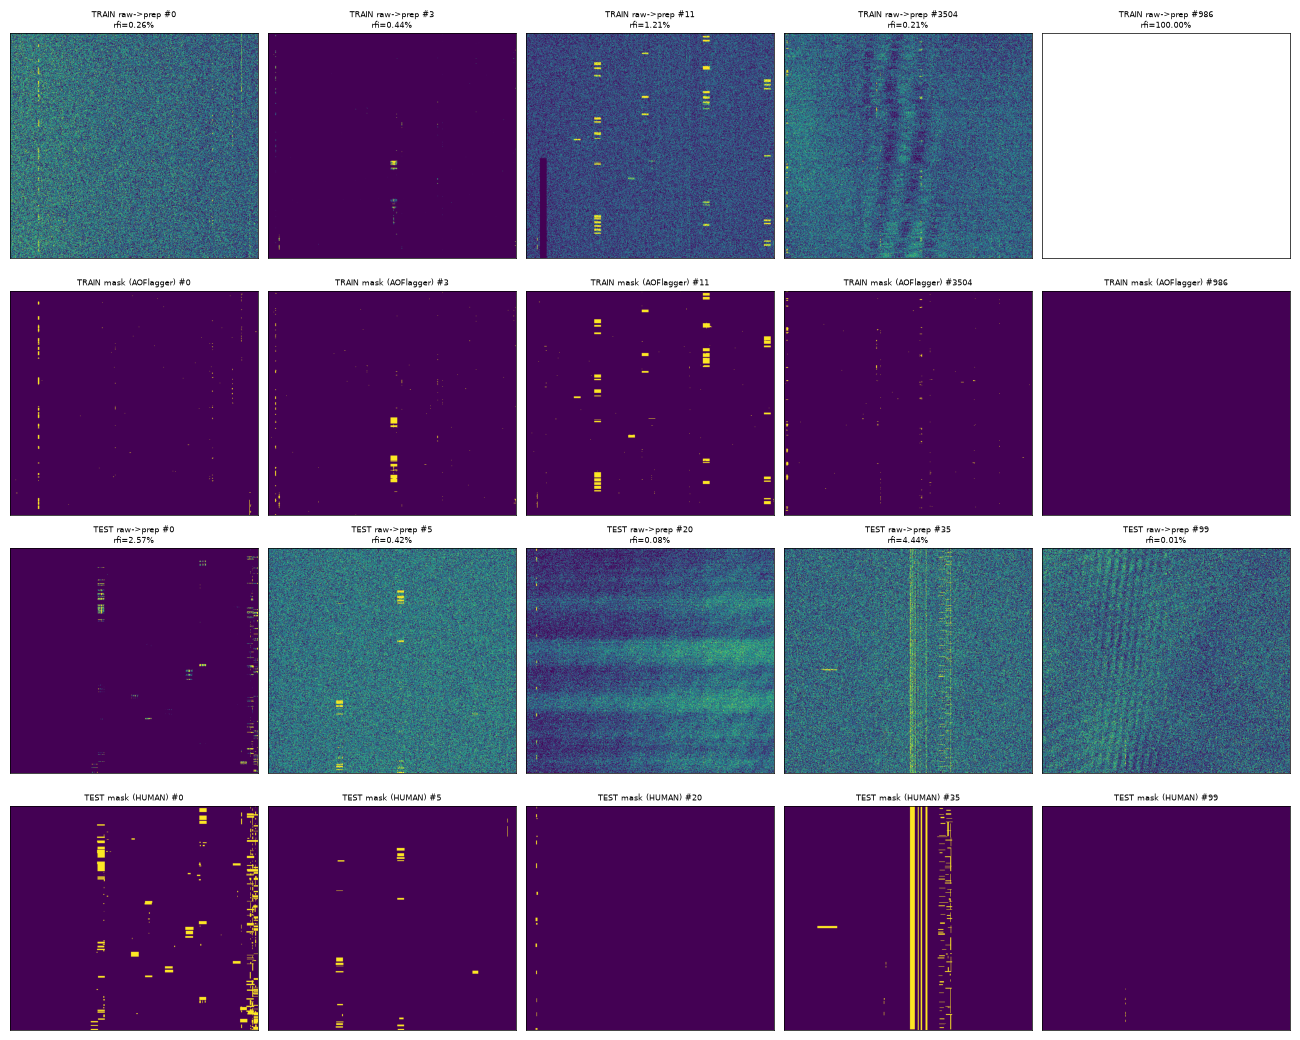
\includegraphics[width=\textwidth]{fig_lofar_overview}
  \caption{Example LOFAR spectrograms (after clipping and log scaling for
    display) and their masks. Top two rows: training images with their
    \aoflagger{} masks; bottom two rows: test images with the human expert's
    masks. Vertical lines are RFI at fixed frequencies.}
  \label{fig:lofar_overview}
\end{figure}

\subsection{Why LOFAR is harder than the synthetic data}
\label{sec:lofar_harder}
LOFAR is harder than the synthetic data for three measurable reasons.

\paragraph{RFI is much rarer.} RFI covers 0.766\% of the pixels in the test
set (1.27\% in the training set), compared with about 15\% in the synthetic
data---roughly one RFI pixel for every 129 clean ones, against one in six. A
model that predicts ``no RFI'' everywhere would be 99.23\% accurate on the test
set while finding nothing, which is why accuracy is not used as a measure
in this report.

\paragraph{Much of the RFI is faint.} In the synthetic data every labelled
pixel is, by construction, above the noise (\cref{sec:synthetic_label}). In
LOFAR that is not true. To measure this I compared each RFI pixel with the
clean pixels of the same image: for each test image I found the 50th, 75th and
99th percentiles of its clean pixels, and placed each RFI pixel into a tier
according to where its brightness falls (\cref{tab:lofar_tiers}). Half of the
RFI is brighter than 99\% of the clean pixels and easy to see, but a fifth of
it is dimmer than a typical clean pixel. Those pixels carry no brightness
evidence at all; they can only be recognised from their surroundings.

\begin{table}[H]
  \centering
  \caption{Brightness of the human-labelled RFI pixels in the 109 LOFAR test
    images, measured against the clean pixels of the same image.}
  \label{tab:lofar_tiers}
  \begin{tabular}{llrr}
    \toprule
    Tier & Brightness relative to the image's clean pixels & RFI pixels & Share \\
    \midrule
    Bright    & above the 99th percentile          & 109{,}669 & 50.1\% \\
    Moderate  & between the 75th and 99th          &  41{,}263 & 18.9\% \\
    Faint     & between the 50th and 75th          &  24{,}113 & 11.0\% \\
    Invisible & below the median                   &  43{,}866 & 20.0\% \\
    \bottomrule
  \end{tabular}
\end{table}

\paragraph{The training labels are often wrong.} Because every test image also
appears in the training set, the \aoflagger{} mask and the human mask can be
compared on exactly the same pixels. Taking the human as correct, \aoflagger{}
has a precision of 0.560 and a recall of 0.580, an \Fone{} of 0.5698. Roughly
44\% of what any model learns from the training labels therefore disagrees
with the expert. As a check on my processing, Mesarcik et al.\ report the same
\aoflagger{} \Fone{} of 0.5698 in their paper\footcite{mesarcik2022}; my value,
0.5698403, agrees to four decimal places, which confirms that I am using the
same test data, labels and metric.

\chapter{Reproducing and diagnosing \tfunet}
\label{ch:tfunet}

\section{Initial result}
The first step was to reproduce the authors' method. I used their \tfunet{}
code without modifying the network itself, with 3 layers and 32 features in
the first layer (465{,}986 trainable parameters), and trained it on the
276$\times$600 synthetic dataset. Two settings had to differ from the paper.
Akeret et al.\ used a batch of 32 images and momentum gradient descent with a
learning rate of 0.2\footcite{akeret2017}. A batch of 32 does not fit on the
6\,GB GPU used here, so I used a batch of 4. At such a small batch the paper's
learning rate destroyed the network within a few iterations (with a batch of
one it stopped learning at iteration 4), so I used the Adam optimiser with a
learning rate of $10^{-3}$ instead.

The result was poor: a maximum \Fone{} of only 0.3879 on the test set, while my
own model (\cref{ch:hybrid}) scored about 0.98 on the same data. The obvious
conclusion would have been that the authors' architecture is simply weaker.
My first suspicion was the normalisation of the input images. Rather than
assume either explanation, I ran a set of controlled experiments.

\section{Four controlled runs}
In four runs everything was kept the same---dataset, network, optimiser and
batch size---except two settings: how the input images were normalised, and
whether class weighting was used (\cref{tab:tfunet_runs},
\cref{fig:tfunet_runs}). Class weighting gives the rare RFI pixels a larger
weight in the loss, and had been added by us to deal with the imbalance
between RFI and clean pixels; it is not part of the authors' setup.

\begin{table}[H]
  \centering
  \caption{\tfunet{} on the 276$\times$600 synthetic dataset. Only the
    normalisation and the class weighting change between runs.}
  \label{tab:tfunet_runs}
  \setlength{\tabcolsep}{4pt}
  \small
  \begin{tabular}{clcrrrl}
    \toprule
    Run & Normalisation & Class weights & Epochs & ROC AUC & max \Fone{} & Behaviour \\
    \midrule
    1 & per-image   & on  & 22 & 0.6681 & 0.3879 & frozen for 15 epochs \\
    2 & per-image   & on  & 5  & 0.5677 & 0.3064 & collapsed, stopped \\
    3 & per-image   & off & 60 & 0.8747 & 0.7191 & trained normally \\
    4 & fixed range & off & 60 & 0.9908 & 0.9317 & trained well \\
    \bottomrule
  \end{tabular}
\end{table}

\begin{figure}[H]
  \centering
  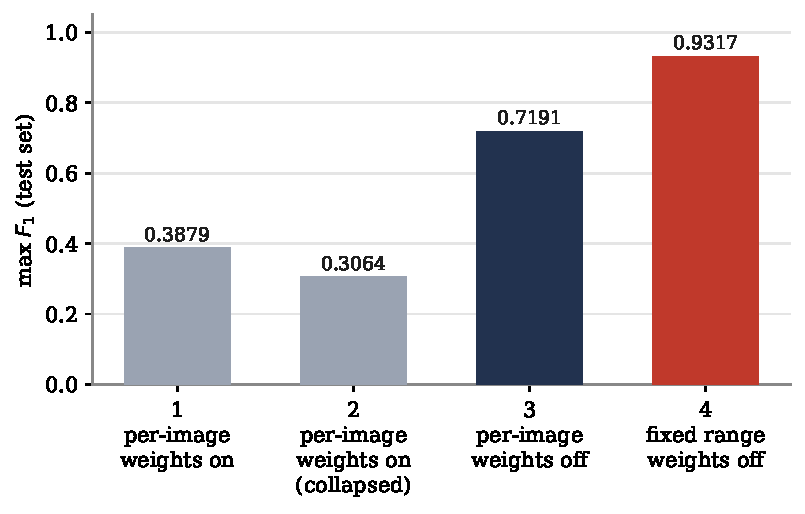
\includegraphics[width=0.75\textwidth]{tfunet_controlled_runs}
  \caption{Test \Fone{} of the four controlled \tfunet{} runs of
    \cref{tab:tfunet_runs}. The network is identical in all four.}
  \label{fig:tfunet_runs}
\end{figure}

Removing the class weights and switching to a fixed normalisation range raised
the score from 0.3879 to 0.9317 without any change to the network. Runs 3 and
4 differ only in normalisation and were trained for the same number of epochs,
so the gain from normalisation alone, $+0.213$, is a fair comparison. The
effect of class weighting is less cleanly separated: run~2 was stopped at
epoch~5 by an automatic check that detects a collapsed network, and run~1
after 22 epochs, while runs 3 and 4 trained for 60. As
\cref{sec:tfunet_v4} shows, a frozen network can eventually recover if
trained for longer, so part of the difference between runs 1--2 and run~3 is
due to training length. What the runs establish clearly is that the poor
initial score came from these two settings, not from the architecture.

\section{Cause 1: class weighting and the ReLU output}
\label{sec:relu_trap}
For every pixel, \tfunet{} produces two scores, one for ``clean'' and one for
``RFI'', and passes both through a ReLU before turning them into
probabilities. A ReLU replaces any negative value with zero. Class weighting
pushes the network strongly towards predicting RFI, which drives the
``clean'' score negative. The ReLU then sets it to exactly zero, and because
the slope of a ReLU is zero for negative inputs, no gradient flows back: the
network has no signal telling it how to change that score. It stops learning.

This is exactly what run~2 shows. It gave the same output, 0.537, for every
one of the 24{,}840{,}000 test pixels. Working backwards through the softmax,
$\mathrm{softmax}(0, c)_2 = 0.537$ gives $c = 0.148$: the ``clean'' score was
stuck at zero and the ``RFI'' score at 0.148 everywhere. The network had become
a constant.

Neither part is a problem on its own. The authors trained successfully with
the ReLU, and class weighting is a standard remedy for imbalanced data. It is
the combination that causes the network to freeze. The freeze is long rather
than permanent: on the second synthetic dataset the same network stayed frozen
for 15 epochs and then began to recover (\cref{sec:tfunet_v4}).

\section{Cause 2: per-image normalisation}
\label{sec:pernorm}
The data loader we had written scaled each image by its own minimum and
maximum. In this dataset the maximum value of an image ranges from 27 to 222,
a factor of 8.2. The same physical brightness therefore ends up at different
values in different images. \Cref{tab:pernorm} shows what this does to a noise
pixel (raw value 10) and a faint RFI pixel (raw value 20).

\begin{table}[H]
  \centering
  \caption{Normalised values of the same two pixels under per-image and
    fixed-range normalisation.}
  \label{tab:pernorm}
  \small
  \begin{tabular}{lccc}
    \toprule
    Pixel (raw value) & Per-image, quiet image & Per-image, bright image & Fixed range \\
     & (max 27) & (max 222) & \\
    \midrule
    Noise (10)     & 0.370 & 0.045 & 0.345 \\
    Faint RFI (20) & 0.741 & 0.090 & 0.520 \\
    \bottomrule
  \end{tabular}
\end{table}

With per-image scaling, noise in the quiet image (0.370) appears brighter than
real RFI in the bright image (0.090), so no single threshold separates RFI from
noise across all images. A fixed range keeps the ordering. The authors had
avoided this problem: their own launch script clips every image to the same
fixed range (from 30 to 210), but this was lost when their code was adapted to
our data. \tfunet{} has no normalisation layers inside the network, so it
cannot correct for it.

The fix was to scale all images with one fixed range, taken as the 0.5th and
99.5th percentiles of the pixel values, averaged over 40 training images
(giving $-9.69$ and $47.40$). Percentiles are used rather than the minimum and
maximum because a single extreme pixel can move the minimum or maximum a long
way. Only training images are used, so no information from the test set
enters the normalisation.

\section{The bandpass dataset}
\label{sec:tfunet_v4}
I repeated the two extreme settings on the 1024$\times$265 dataset with the
instrument bandpass. With per-image normalisation and class weights, the
network stayed frozen at a validation \Fone{} of about 0.37 for the first 15
epochs, then escaped and kept improving until the last epoch, finishing at a
test \Fone{} of 0.6815. With a fixed range and no class weights it reached
0.9483 and had converged by epoch 30. The same two settings decide the result
on the harder dataset too.

\section{\tfunet{} on real LOFAR data}
\label{sec:tfunet_lofar}
Having found the settings that make \tfunet{} work on synthetic data, I trained
it on the real LOFAR data with exactly those settings: the unmodified network,
fixed-range normalisation and no class weighting. The model was trained on the
6621 clean training images, the threshold was chosen on the 735 validation
images, and the result was measured on the 109 images labelled by the human
expert. Each setting was run with three random seeds.

Despite the extreme imbalance---one RFI pixel for every 129 clean ones---the
network did not collapse into predicting ``no RFI'' everywhere. With the same
training length as on the synthetic data (60 epochs at a learning rate of
$10^{-3}$) it reached a maximum \Fone{} of $0.4901 \pm 0.0495$. Lowering the
learning rate to $10^{-4}$ and training for 150 epochs raised this to
$0.5482 \pm 0.0139$ (\cref{tab:tfunet_lofar}).

\begin{table}[H]
  \centering
  \caption{\tfunet{} on the 109 human-labelled LOFAR test images. Mean and
    standard deviation over three seeds.}
  \label{tab:tfunet_lofar}
  \begin{tabular}{lccc}
    \toprule
    Training & max \Fone{} & pooled \Fone{} & ROC AUC \\
    \midrule
    lr $10^{-3}$, 60 epochs  & $0.4901 \pm 0.0495$ & $0.4563 \pm 0.0279$ & $0.9389 \pm 0.0045$ \\
    lr $10^{-4}$, 150 epochs & $0.5482 \pm 0.0139$ & $0.5021 \pm 0.0259$ & $0.9470 \pm 0.0074$ \\
    \bottomrule
  \end{tabular}
\end{table}

The lower learning rate also made the result much more consistent between
seeds: the standard deviation of the maximum \Fone{} fell from 0.0495 to
0.0139. However, the improvement itself is not statistically significant with
three seeds. Comparing the runs seed by seed, one of the three seeds actually
became slightly worse, and a paired $t$-test gives $t = 1.54$ with 2 degrees of
freedom, well below the 4.30 needed for significance at the 5\% level. My
first single run had suggested a gain of 0.118; the two further seeds roughly
halved it. I therefore use the lower learning rate as the better default, but
do not claim it as a proven improvement.

Using per-image normalisation instead, the maximum \Fone{} fell to 0.3039, below
even a simple threshold, which confirms on real data the conclusion of
\cref{sec:pernorm}.

\Cref{fig:tfunet_lofar} places the result among published methods. The values
for Mesarcik et al.'s U-Net and for RFI-Net are taken from their
paper\footcite{mesarcik2022}; I did not re-run those methods. Their results are
reported as maximum \Fone{}, which is why that measure is used here.
\tfunet{} clearly beats a simple $\sigma$-clipping threshold (0.4103) but stays
below \aoflagger{} (0.5698), and is 0.039 below Mesarcik et al.'s U-Net (0.5876).
Two known differences in how that U-Net was trained could account for at least
part of the gap: it was trained on small 32$\times$32 patches rather than full
images, and with a different normalisation. I have not tested which of these
matters.

\begin{figure}[H]
  \centering
  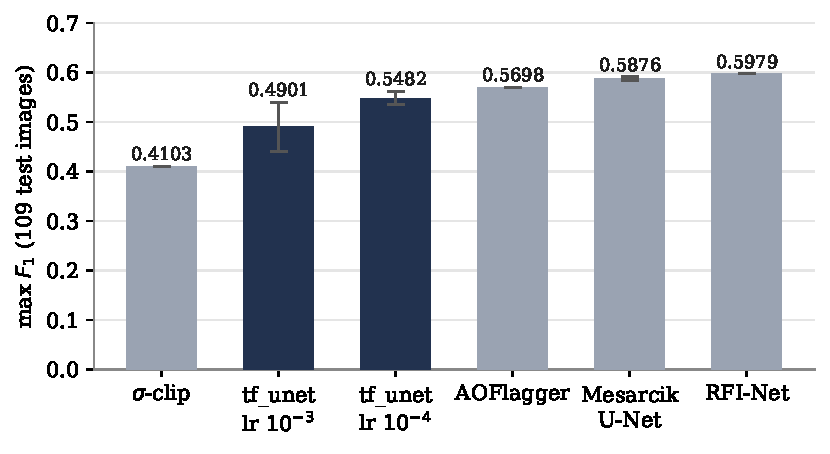
\includegraphics[width=0.8\textwidth]{tfunet_lofar_ladder}
  \caption{Maximum \Fone{} on the 109 LOFAR test images. Dark bars are my
    \tfunet{} runs (error bars: standard deviation over three seeds); grey bars
    are a $\sigma$-clipping threshold, \aoflagger{}, and the values reported by
    Mesarcik et al.}
  \label{fig:tfunet_lofar}
\end{figure}

\section{From synthetic to real data}
\label{sec:gap}
The same network, trained with the same settings and the same number of
gradient steps (10{,}500), scores 0.9317 on the synthetic data and 0.4901 on
LOFAR: a drop of 0.44 in \Fone{}. Even the best LOFAR result, after tuning the
learning rate, is 0.38 below the synthetic score. The reasons were set out in
\cref{sec:lofar_harder}: real RFI is far rarer, much of it is fainter than the
noise, and the training labels themselves are often wrong. A method that
performs well on a synthetic benchmark can therefore perform much worse on
real observations, and synthetic results alone should be read with care.

\chapter{\hybrid}
\label{ch:hybrid}
Alongside reproducing \tfunet{}, I designed a second network, which I call
\hybrid{}. It keeps the same overall U-Net shape but combines several
components that other RFI and segmentation work has used, chosen with the
properties of RFI in mind. This chapter describes the model and its results;
\cref{ch:drivers} then tests which of its components actually matter.

\section{Design}
\label{sec:hybrid_design}
The starting point was an observation about the synthetic data: after
normalisation, faint RFI sits only about 1.5 noise standard deviations above
the background. At that level a single pixel cannot be told apart from a
noise fluctuation. A faint narrowband line is detectable only because it
extends over many time samples, not because any one pixel is bright. Most of
the design choices were aimed at using this kind of spatial context.

\Cref{tab:hybrid_vs_tfunet} lists how the model differs from \tfunet{}.

\begin{table}[H]
  \centering
  \caption{Differences between \tfunet{} and \hybrid{}.}
  \label{tab:hybrid_vs_tfunet}
  \begin{tabular}{p{3.4cm}p{4.3cm}p{5.2cm}}
    \toprule
    Component & \tfunet{} & \hybrid{} \\
    \midrule
    Convolution blocks & two 3$\times$3 convolutions & residual blocks (with a shortcut path) \\
    Line-shaped filters & none & multi-scale strip convolutions \\
    Channel attention & none & efficient channel attention (ECA) \\
    Normalisation layers & none & GroupNorm after each convolution \\
    Output layer & ReLU, then softmax & raw scores, then softmax \\
    Padding & valid (output smaller than input) & same (output = input size) \\
    Depth / first-layer width & 3 levels / 32 & 4 levels / 8 \\
    Loss & cross-entropy & cross-entropy + Dice \\
    Framework & TensorFlow & PyTorch \\
    Parameters & 465{,}986 & 593{,}842 \\
    \bottomrule
  \end{tabular}
\end{table}

\paragraph{Residual blocks.} Each block adds its input back to its output
through a shortcut\footcite{he2016}, so a feature only has to learn a correction
rather than be rebuilt at every layer. The aim was to stop weak, low-contrast
features being washed out as they pass through many layers. RFI-Net, the best
method in Mesarcik et al.'s comparison, is also built from residual
blocks\footcite{yang2020rfinet}.

\paragraph{Multi-scale strip convolutions.} Ordinary filters are small
squares, but much RFI is line-shaped: narrowband RFI is a thin line along the
time axis, and a wideband burst a thin line along the frequency axis. A strip
filter of size $1\times K$ or $K\times1$ adds up the signal along such a line.
Averaging $K$ pixels of a coherent line improves its signal-to-noise ratio by
about $\sqrt{K}$, while noise averages down, which is how a 1.5$\sigma$ line
could become detectable. Filters of three lengths ($K = 7, 11, 21$) run in
parallel to cover RFI of different durations and bandwidths. Multi-scale
convolutions of this kind have been used for RFI before\footcite{gu2024emsca}, and
a closely related strip-convolution design has since been
published\footcite{mars2026}, so this component is not new.

\paragraph{Efficient channel attention.} After the strip filters, some feature
channels carry evidence of faint RFI and others of bright RFI. ECA\footcite{wang2020eca}
learns a weight for each channel at very little cost (a single small
one-dimensional convolution), so that the faint-structure channels are not
drowned out by the bright ones.

\paragraph{GroupNorm.} Normalisation layers rescale the values inside the
network so that they stay in a stable range. A common choice, batch
normalisation, estimates its statistics across the images in a batch, which is
unreliable when, as here, the GPU memory allows only one 512$\times$512 image
per batch. GroupNorm\footcite{wu2018groupnorm} computes its statistics within a
single image and so works at any batch size. \tfunet{} has no normalisation
layers at all.

\paragraph{No ReLU on the output.} \hybrid{} passes its raw output scores
directly to the softmax. This removes the failure described in
\cref{sec:relu_trap}, where class weighting and an output ReLU freeze
\tfunet{}.

\paragraph{Same padding.} The output has the same size as the input, so every
pixel of the 512$\times$512 image receives a prediction. With \tfunet{}'s valid
padding, a border around each image is lost.

\section{Training}
\label{sec:hybrid_training}
The model is trained with the sum of two losses. Cross-entropy scores each
pixel separately. The Dice loss\footcite{milletari2016} measures how well the
predicted RFI region overlaps the true one as a whole, which helps when the
positive class is rare, as RFI is in LOFAR. I used the Adam optimiser with a
learning rate of $10^{-3}$ and one image per batch, for 40 epochs of 700 steps
(28{,}000 gradient steps). As for \tfunet{}, the input is scaled with a fixed
range measured on training images only, and the best checkpoint and the
decision threshold are chosen on the 735 validation images.

\section{Results on synthetic data}
On the synthetic data the model performs very well, but as
\cref{sec:gap} showed, this data is much easier than real observations, so
these results are mainly a check that the model trains correctly.
On the 276$\times$600 dataset a wide version of the model (32 filters in the
first layer, 9{,}304{,}186 parameters) reached an \Fone{} of 0.9808, and on the
1024$\times$265 dataset the narrow version used in the rest of this report (8
filters, 593{,}842 parameters) reached 0.9878. These values use a threshold
chosen on the validation set.

The width of the network can be reduced a long way at little cost
(\cref{tab:width}). Going from 32 to 8 filters in the first layer removes 94\%
of the parameters and lowers \Fone{} by only 0.006; only at 4 filters does the
model clearly get worse. Each width was trained once, so differences of less
than about 0.01 should not be over-interpreted.

\begin{table}[H]
  \centering
  \caption{Effect of network width on the 276$\times$600 synthetic dataset
    (one run each).}
  \label{tab:width}
  \begin{tabular}{rrr}
    \toprule
    First-layer filters & Parameters & \Fone{} \\
    \midrule
    4  & 152{,}582     & 0.9547 \\
    8  & 593{,}842     & 0.9749 \\
    16 & 2{,}342{,}474 & 0.9788 \\
    32 & 9{,}304{,}186 & 0.9812 \\
    \bottomrule
  \end{tabular}
\end{table}

\section{Results on LOFAR}
\label{sec:hybrid_lofar}

\subsection{Class weighting}
I first trained the model on LOFAR with class weighting, giving RFI pixels 57
times the weight of clean ones to balance their rarity. Over three seeds it
reached a maximum \Fone{} of $0.6467 \pm 0.0079$. However, the threshold chosen
on the validation set was 0.96, far from the usual 0.5: the weighting pushed
the model's outputs so high that only near-certain predictions could be
trusted. Without class weighting, the score rose to $0.6603 \pm 0.0040$ and the
threshold fell to $0.26$. Removing the weight improved the result for every one
of the three seeds (by 0.009 to 0.016; paired $t = 6.03$ with 2 degrees of
freedom, significant at the 5\% level), so the unweighted model is used from
here on.

Interestingly, the area under the ROC curve moved the opposite way, falling
from 0.980 to 0.938. The ROC curve measures how well the model ranks RFI pixels
above clean ones, while \Fone{} measures the quality of the final yes/no
decision. Class weighting improved the ranking but made the decisions worse,
which shows that a high ROC area alone does not mean a model flags RFI well.

\subsection{Comparison with published methods}
\Cref{tab:final} and \cref{fig:final} compare the final model with the other
methods on the 109 human-labelled test images. \hybrid{} reaches a maximum
\Fone{} of $0.6603 \pm 0.0040$, which is 0.062 above RFI-Net (0.5979), the best
result reported by Mesarcik et al.; this difference is significant
(one-sample $t = 27.2$ with 2 degrees of freedom). With the threshold fixed in
advance on the validation set, the pooled \Fone{} is $0.6561 \pm 0.0044$. It
also scores 0.11 above \tfunet{}, and it does so while having been trained on
\aoflagger{}'s labels, which themselves score only 0.5698 against the human
expert: the model ends up agreeing with the expert more than its own training
labels do. It is the highest score of all the methods compared in this report:
above Akeret et al.'s \tfunet{} (0.5482), Mesarcik et al.'s U-Net (0.5876) and
RFI-Net (0.5979).

\begin{table}[H]
  \centering
  \caption{Results on the 109 human-labelled LOFAR test images. Values for
    Mesarcik et al.'s U-Net and RFI-Net are as reported in their
    paper.}
  \label{tab:final}
  \begin{tabular}{lcr}
    \toprule
    Method & max \Fone{} & Parameters \\
    \midrule
    $\sigma$-clipping threshold & 0.4103 & --- \\
    \tfunet{} (lr $10^{-4}$, 3 seeds) & $0.5482 \pm 0.0139$ & 465{,}986 \\
    \aoflagger{} & 0.5698 & --- \\
    Mesarcik et al.\ U-Net & $0.5876 \pm 0.0031$ & --- \\
    RFI-Net & 0.5979 & --- \\
    \hybrid{}, class-weighted (3 seeds) & $0.6467 \pm 0.0079$ & 593{,}842 \\
    \textbf{\hybrid{} (3 seeds)} & $\mathbf{0.6603 \pm 0.0040}$ & 593{,}842 \\
    \bottomrule
  \end{tabular}
\end{table}

\begin{figure}[H]
  \centering
  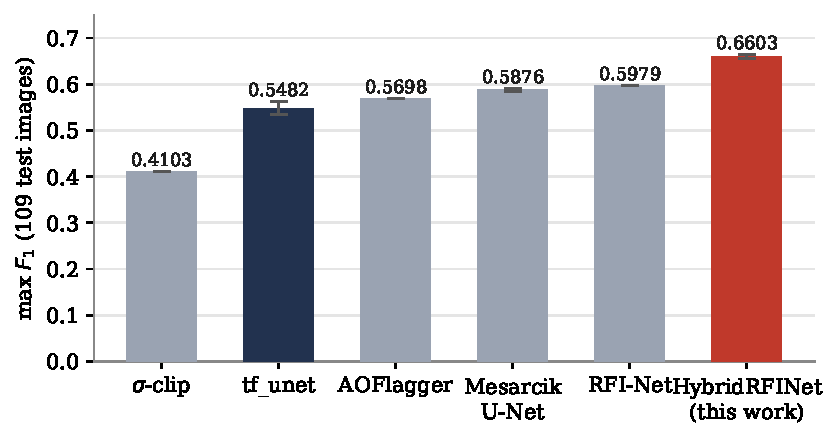
\includegraphics[width=0.8\textwidth]{hybrid_lofar_ladder}
  \caption{Maximum \Fone{} on the 109 LOFAR test images. Error bars show the
    standard deviation over three seeds where available.}
  \label{fig:final}
\end{figure}

A wider version of the model, with 32 filters and 9.3 million parameters,
scored 0.6571 with class weighting (one run), against $0.6467 \pm 0.0079$ for
the narrow class-weighted model. Fifteen times more parameters therefore buys
very little, consistent with the synthetic results in \cref{tab:width}.

\section{Checking the result}
\label{sec:audit}
Because the result is better than the published state of the art, I checked
it for mistakes before relying on it, using a separate script that shares no
evaluation code with the training script.
\begin{itemize}
  \item \textbf{Metrics recomputed independently} from the saved model agree
    with the reported values to within $3\times10^{-5}$; the remaining
    difference comes from GPU non-determinism.
  \item \textbf{No leakage:} none of the training or validation images appears
    in the test set, and the normalisation range is computed from training
    images only.
  \item \textbf{Honest threshold:} choosing the threshold on the validation set
    costs 0.006 in \Fone{} compared with choosing the best threshold on the
    test set itself; the lower, honest value is the one reported.
  \item \textbf{Little overfitting:} maximum \Fone{} is 0.711 on training
    images, 0.682 on validation and 0.659 on test.
  \item \textbf{Not a copy of \aoflagger{}:} the model agrees with \aoflagger{}
    at an \Fone{} of only 0.743. It finds 16{,}485 true RFI pixels that
    \aoflagger{} missed and misses 7{,}345 that \aoflagger{} found.
  \item \textbf{Not a simple frequency rule:} flagging the 16 most
    RFI-affected frequency channels everywhere scores only 0.065.
  \item \textbf{Robust to the choice of test images:} resampling the 109 test
    images 2000 times (bootstrap) gives a 95\% interval for the pooled \Fone{}
    of $[0.615, 0.692]$; RFI-Net's 0.5979 lies outside it, and 99.5\% of the
    resamples beat it.
\end{itemize}
The width of that interval, about $\pm0.04$, is the largest uncertainty in the
result. It comes from having only 109 test images, not from the model.

\chapter{What drives the performance}
\label{ch:drivers}
\Cref{ch:hybrid} showed that \hybrid{} scores 0.11 above \tfunet{} on LOFAR and
above the best published result. The natural explanation is that the
components added for RFI---the strip convolutions, channel attention and
residual blocks---are responsible. This chapter tests that explanation
directly. It turns out to be wrong.

\section{Removing the components one at a time}
\label{sec:ablation}
To find out what each component contributes, I wrote a version of the network
in which each component can be switched off, and trained every variant
through exactly the same pipeline as the full model: same data, splits,
normalisation, loss, optimiser, number of steps and threshold selection. Only
the network changes. As a check, the switchable network with everything
switched on scored 0.6624, in line with the real model's $0.6603 \pm 0.0040$, so
it faithfully reproduces \hybrid{}.

\Cref{tab:ablation} shows the results. Removing the strip convolutions,
the attention or the residual blocks one at a time changes the score by less
than 0.007, and removing the strip convolutions even raised it slightly.
Removing all three at once (``plain U-Net'') gives 0.6605, essentially the same
as the full model.

\begin{table}[H]
  \centering
  \caption{Ablation on the 109 LOFAR test images (maximum \Fone{}, one seed).
    The seed-to-seed standard deviation of the full model is 0.0040, so
    differences below about 0.008 are within noise.}
  \label{tab:ablation}
  \begin{tabular}{lrrr}
    \toprule
    Variant & Parameters & max \Fone{} & Change \\
    \midrule
    Full model                                   & 593{,}842 & 0.6624 & --- \\
    without strip convolutions                   & 508{,}210 & 0.6637 & $+0.0013$ \\
    without channel attention                    & 593{,}818 & 0.6557 & $-0.0067$ \\
    without residual blocks                      & 572{,}074 & 0.6569 & $-0.0055$ \\
    without all three (plain U-Net)              & 486{,}418 & 0.6605 & $-0.0019$ \\
    plain U-Net without GroupNorm                & 485{,}682 & 0.6289 & $-0.0335$ \\
    \bottomrule
  \end{tabular}
\end{table}

With one run per variant, only the last row looked like a real effect:
removing GroupNorm cost 0.034, more than eight times the seed spread. Because a
single run can mislead (\cref{sec:tfunet_lofar}), I repeated the two most
important variants with two more seeds (\cref{tab:ablation3}).

\begin{table}[H]
  \centering
  \caption{The key ablation variants over three seeds (maximum \Fone{}).}
  \label{tab:ablation3}
  \small
  \begin{tabular}{lcccc}
    \toprule
    Model & Seed 0 & Seed 1 & Seed 2 & Mean $\pm$ s.d. \\
    \midrule
    Full \hybrid{}                 & 0.6592 & 0.6647 & 0.6570 & $0.6603 \pm 0.0040$ \\
    Plain U-Net (three components removed) & 0.6605 & 0.6618 & 0.6531 & $0.6585 \pm 0.0047$ \\
    Plain U-Net without GroupNorm  & 0.6289 & 0.6600 & 0.6595 & $0.6495 \pm 0.0178$ \\
    \bottomrule
  \end{tabular}
\end{table}

The full model and the plain U-Net are not significantly different (Welch
$t$-test, $p = 0.64$): the three components contribute nothing measurable. The
apparent effect of GroupNorm also largely disappeared. The first run without it
was an outlier; the other two scored the same as the plain U-Net, and with
three seeds the difference is not significant ($p = 0.48$). The one clear sign
is that without GroupNorm the results vary about four times more from seed to
seed, so normalisation seems to make training more stable even if it does not
make the final model better on average.

\section{Do the strip convolutions help with faint RFI?}
\label{sec:faint}
The main reason for adding strip convolutions was faint RFI
(\cref{sec:hybrid_design}). Faint RFI is a small share of all RFI pixels, so a
benefit there could be hidden in the overall score. To test this I measured how
much of the RFI in each brightness tier of \cref{tab:lofar_tiers} the model
finds, with and without the strip convolutions.

The first comparison seemed to show a small benefit of about 0.02 in the
fainter tiers. However, each model had been scored at its own threshold, and
these differed (0.30 with strip convolutions, 0.43 without). A lower threshold
flags more pixels and so finds more RFI in every tier, regardless of the
architecture. To remove this effect I set each model's threshold so that both
flag exactly the same number of pixels (199{,}951), and compared again
(\cref{tab:faint}). The difference vanished in every tier, including the
faint and invisible ones the strip convolutions were designed for.

\begin{table}[H]
  \centering
  \caption{Fraction of RFI found in each brightness tier, with both models
    flagging the same number of pixels.}
  \label{tab:faint}
  \begin{tabular}{lrrr}
    \toprule
    Tier & With strip conv. & Without & Difference \\
    \midrule
    Bright    & 0.940 & 0.945 & $-0.005$ \\
    Moderate  & 0.405 & 0.402 & $+0.003$ \\
    Faint     & 0.273 & 0.274 & $-0.001$ \\
    Invisible & 0.258 & 0.257 & $+0.001$ \\
    \bottomrule
  \end{tabular}
\end{table}

The table also shows where the model's errors are. Bright RFI is almost
entirely found (94\%), but only about a quarter of the faint and invisible RFI
is, so most of the RFI the model misses is dim.

\section{Adding a CRF refinement}
\label{sec:crf}
Chen et al.\footcite{chen2023} clean RFI in pulsar data by first labelling pixels
with a simple statistical threshold and then refining the labels with a
conditional random field (CRF), which adjusts each pixel's label according to
its neighbours. They report that this recovers weak RFI that is unrecognisable
in individual pixels but visible from its surroundings---exactly the faint RFI
my model misses. I therefore added a CRF on top of the trained network. I
implemented it as differentiable layers\footcite{zheng2015crfrnn,teichmann2018convcrf},
so that its settings can also be learned, and gave it separate ranges along
time and frequency. It adds only 11 parameters.

\begin{table}[H]
  \centering
  \caption{Adding a CRF to the trained network (maximum \Fone{}, 109 LOFAR test
    images).}
  \label{tab:crf}
  \begin{tabular}{lr}
    \toprule
    Configuration & max \Fone{} \\
    \midrule
    Network alone                                  & 0.6592 \\
    + CRF with Chen et al.'s settings              & 0.4884 \\
    + CRF with the best hand-chosen settings       & 0.6604 \\
    + CRF with settings learned in training        & 0.6604 \\
    \bottomrule
  \end{tabular}
\end{table}

With Chen et al.'s published settings the CRF was harmful
(\cref{tab:crf}): it removed isolated detections whose neighbours were labelled
clean, raising precision to 0.74 but cutting recall to 0.35. Their RFI arrives
in large connected blocks, while LOFAR RFI is sparse and thin. With better
settings, whether chosen by hand or learned, the gain was 0.0012, well inside
the seed spread. When the CRF was free to learn how strongly to act, it reduced
its own weights towards zero (the setting at which it changes nothing) and
stopped improving after the second of 40 epochs.

There are two reasons it does not help here. The network already uses the
neighbourhood of each pixel through its convolutions, so the CRF has little to
add; Chen et al.\ applied theirs to a simple threshold that uses no
neighbourhood information at all. And a CRF can only rearrange evidence that is
already in the network's prediction; for faint RFI there is very little such
evidence to rearrange.

\section{What explains the gain over \tfunet{}?}
\label{sec:unexplained}
Taken together, these results show that the gain of \hybrid{} over \tfunet{}
does not come from the components it was designed around. A plain U-Net with
the same training setup scores almost as well. What remains are the other
differences listed in \cref{tab:hybrid_vs_tfunet}: the Dice loss, the output
layer without a ReLU, same padding, the different depth and width, batch size,
learning rate and framework. I have not yet tested these one by one, so I
cannot say which of them is responsible. The natural first test is to train
the plain U-Net without the Dice loss.

\chapter{Discussion}
\label{ch:discussion}

\section{What worked, and what did not}
The clearest result of this project is negative, and it repeated itself. Several
choices that looked as though they should help turned out not to, and in each
case this became visible only through a controlled test.

\begin{itemize}
  \item \tfunet{}'s poor first score looked like a weakness of its architecture.
    It came instead from two training settings, class weighting and per-image
    normalisation; correcting them took it from 0.39 to 0.93 without changing
    the network (\cref{ch:tfunet}).
  \item The components \hybrid{} was designed around---strip convolutions,
    channel attention and residual blocks---contribute nothing measurable on
    real data, not even for the faint RFI they were meant to target
    (\cref{ch:drivers}).
  \item A CRF refinement that works well on top of a simple threshold added
    nothing on top of a network that already uses neighbourhood information,
    and with its published settings it was harmful (\cref{sec:crf}).
\end{itemize}

The model still beats the best published result on LOFAR, but the reason is
not the one it was designed around. Without the ablation, I would have
credited the wrong parts of the model.

\section{Synthetic benchmarks can mislead}
The same network, trained the same way, scored 0.93 on my synthetic data and
0.49 on LOFAR. The synthetic labels are noise-free and every labelled pixel is
above the noise by construction, while on real data a fifth of the RFI is
fainter than a typical clean pixel and the training labels disagree with a
human expert about 44\% of the time. The synthetic data was useful for finding
and fixing \tfunet{}'s training problems quickly, but it was a poor guide to
how methods compare on real observations: on synthetic data every variant of
my model scored above 0.95, so it could not show which parts mattered.

\section{Single runs can mislead}
Three times in this project, an effect measured with one training run shrank
or disappeared when the run was repeated with different random seeds:
\begin{itemize}
  \item lowering \tfunet{}'s learning rate first appeared to add 0.118 to
    \Fone{}; over three seeds the mean gain was 0.058 and not significant
    (\cref{sec:tfunet_lofar});
  \item removing GroupNorm first appeared to cost 0.034; over three seeds the
    difference was 0.009 and not significant (\cref{sec:ablation});
  \item strip convolutions first appeared to help faint RFI by about 0.02; the
    effect came from comparing models at different thresholds and vanished
    when they were compared fairly (\cref{sec:faint}).
\end{itemize}
On LOFAR, results vary between seeds by up to about 0.05 in \Fone{}, which is as
large as many of the effects one might want to measure. Repeating runs and
comparing models under identical conditions was the only reliable way to tell
real effects from noise.

\section{Limitations}
\begin{enumerate}
  \item \textbf{Published baselines are quoted.} The results for
    Mesarcik et al.'s U-Net and RFI-Net are taken from their
    paper\footcite{mesarcik2022}. Because my measurement of \aoflagger{} matches
    theirs to four decimal places, the test data, labels and metric are the
    same, so the comparison is like for like; the values themselves are as
    they reported them.
  \item \textbf{Small test set.} There are only 109 human-labelled test images.
    The resulting uncertainty, about $\pm0.04$ in \Fone{} at 95\% confidence, is
    larger than the variation between seeds.
  \item \textbf{Different training budgets.} Mesarcik et al.\ trained on
    32$\times$32 patches for 100 epochs; I trained on full images for a fixed
    number of steps. Each method was trained in a sensible way for it, but not
    under one common budget.
  \item \textbf{Three seeds.} This is the minimum for any statistical
    statement, and several conclusions rest on it.
  \item \textbf{One real dataset.} All real-data results come from LOFAR. The
    method has not been tested on data from another telescope, including the
    GMRT data that originally motivated this project.
  \item \textbf{The gain over \tfunet{} is not yet explained}
    (\cref{sec:unexplained}).
  \item \textbf{\tfunet{} was not run on HERA}, so it is compared with my model
    only on the synthetic data and on LOFAR.
\end{enumerate}

\section{Future work}
The results suggest that further additions to the model should target a
specific, measured weakness, and each should be tested by removing it again.
\begin{itemize}
  \item \textbf{Find the source of the current gain.} Train the plain U-Net
    without the Dice loss, then test the other remaining differences from
    \tfunet{} one at a time. This is cheap and would explain the main result.
  \item \textbf{Reduce false alarms.} False positives are the largest single
    source of error: if all were removed, \Fone{} would rise from about 0.65 to
    0.77. Losses or post-processing aimed specifically at precision are a
    natural next step.
  \item \textbf{Learn from noisy labels.} Every training label comes from
    \aoflagger{}, which disagrees with the human expert on about 44\% of RFI.
    Methods designed for training with noisy labels could help more than
    further changes to the architecture.
  \item \textbf{Faint RFI.} Only about a quarter of the faint and invisible RFI
    is found. Since these pixels carry no brightness signal of their own, any
    improvement has to come from wider context.
  \item \textbf{Apply the method to GMRT pulsar data}, the original motivation
    for this project.
\end{itemize}

\chapter{Conclusion}
\label{ch:conclusion}
This project set out to apply U-Net-based RFI detection, first by reproducing
the method of Akeret et al.\ and then by designing an improved network, and to
test both on real telescope data rather than only on synthetic data.

The authors' \tfunet{} first scored an \Fone{} of 0.39 on my synthetic data.
Controlled experiments showed that this was caused by two training settings,
class weighting combined with the network's ReLU output layer, and per-image
normalisation, and not by its architecture. Correcting them raised the score to
0.93 without changing the network.

On real LOFAR data labelled by a human expert, the corrected \tfunet{} reached
a maximum \Fone{} of $0.5482 \pm 0.0139$, close to the U-Net result published for
the same data. My network, \hybrid{}, reached $0.6603 \pm 0.0040$ with under
600{,}000 parameters, above the best published result of 0.5979. Independent
checks found no leakage or evaluation error behind this result.

Removing the strip convolutions, channel attention and residual blocks that
\hybrid{} was designed around did not measurably change its score, and adding
a CRF refinement did not improve it. The advantage over \tfunet{} therefore
comes from other differences in the network and its training, which remain to
be identified.

Along the way, checking the public HERA and LOFAR datasets showed that both
contain test images that also appear in the training set, and comparing the
same network on synthetic and real data showed a drop of 0.44 in \Fone{}. Both
point to the same lesson as the rest of this work: results need to be checked
on real data, with repeated runs, before their explanations can be trusted.


% Note:
% Use sections/subsections to structure content within each chapter.

%=========================================================================================
% APPENDICES
%=========================================================================================

\appendix
\appendixpage
\addappheadtotoc
\chapter{Reproducibility}
\label{app:repro}

\section{Computing environment}
The work began on Windows 11 using the Windows Subsystem for Linux (WSL2). WSL2
by default makes only about half of the system memory available to Linux,
roughly 9\,GB of the 19\,GB here, which is less than the 9.3\,GB LOFAR file. On
my supervisor's advice the project was moved to a native Linux installation.
(Raising WSL2's memory limit in its configuration file would also have solved
this particular problem.) \Cref{tab:env} lists the final environment.

\begin{table}[H]
  \centering
  \caption{Computing environment.}
  \label{tab:env}
  \begin{tabular}{ll}
    \toprule
    Component & Version \\
    \midrule
    Operating system & Fedora 44, kernel 6.19.10 \\
    GPU & NVIDIA RTX 3060 Laptop, 6\,GB \\
    Driver / CUDA & 610.57.04 / 13.3 \\
    \tfunet{} environment & Python 3.12, TensorFlow 2.21.0 \\
    \hybrid{} environment & Python 3.14, PyTorch 2.13.0 \\
    \bottomrule
  \end{tabular}
\end{table}

TensorFlow and PyTorch need incompatible versions of NVIDIA's cuDNN library, so
they are kept in two separate Python environments. Training speed depends
strongly on power: on battery the GPU is throttled to 210\,MHz of its 2100\,MHz,
and one \tfunet{} training step took 2684\,ms instead of 174\,ms---15 times
slower.

\section{Code and data}
All code, analysis scripts and per-run metrics are in the project repository,
\url{https://github.com/RonakSinghRaina/MP}. The HERA and LOFAR datasets are
available from Zenodo\footcite{mesarcik2022data}; the synthetic datasets are
regenerated from the generator with seed 42. The main experiments are run with:
\begin{lstlisting}[language=bash]
# tf_unet on LOFAR (TensorFlow environment)
~/tf-env/bin/python experiments/lofar_tfunet_baseline.py --lr 1e-4 --epochs 150 --seed 0

# HybridRFINet on LOFAR (PyTorch environment)
~/torch-env/bin/python experiments/lofar_hybrid.py --base 8 --no_class_weight --seed 0

# Ablation: any variant through the same pipeline
~/torch-env/bin/python experiments/lofar_hybrid.py --variant plain_unet \
    --base 8 --no_class_weight --seed 0
\end{lstlisting}


%=========================================================================================
% BIBLIOGRAPHY
%=========================================================================================

\nocite{*}                               % Include all entries from ref.bib
\printbibliography[heading=bibintoc]     % Bibliography in ToC

\end{document}